\documentclass[11pt,a4paper]{article}
\usepackage[margin=2.2cm]{geometry}
\usepackage{lmodern}
\usepackage[T1]{fontenc}
\usepackage[utf8]{inputenc}
\usepackage{amsmath,amssymb}
\usepackage{booktabs,array,tabularx,longtable}
\usepackage{enumitem}
\usepackage{xcolor}
\usepackage[most]{tcolorbox}
\usepackage{titlesec}
\usepackage{graphicx}
\usepackage{float}
\usepackage{adjustbox}
\usepackage{tikz}
\usetikzlibrary{arrows.meta,positioning,calc}
\usepackage[font=small,labelfont={bf,color=headblue},skip=4pt]{caption}
\usepackage[colorlinks=true,linkcolor=headblue,urlcolor=blue!50!black]{hyperref}

\definecolor{headblue}{RGB}{38,70,120}
\titleformat{\part}[display]{\centering\Huge\bfseries\color{headblue}}{Part \thepart}{10pt}{}
\titleformat{\section}{\Large\bfseries\color{headblue}}{\thesection}{0.8em}{}[{\color{black}\titlerule}]
\titleformat{\subsection}{\large\bfseries\color{headblue}}{\thesubsection}{0.8em}{}
\titleformat{\subsubsection}{\normalsize\bfseries\color{headblue}}{\thesubsubsection}{0.8em}{}
\titlespacing*{\section}{0pt}{12pt}{6pt}
\titlespacing*{\subsection}{0pt}{9pt}{3pt}
\setlength{\parindent}{0pt}
\setlength{\parskip}{5pt}
\setlist{itemsep=1pt,topsep=2pt}
\renewcommand{\arraystretch}{1.12}
\setlength{\emergencystretch}{3em}

\newtcolorbox{keybox}{colback=blue!3,colframe=headblue!60,boxrule=0.5pt,arc=2mm,left=2mm,right=2mm,top=1mm,bottom=1mm}
\newtcolorbox{insum}{colback=green!3,colframe=green!40!black,boxrule=0.4pt,arc=1.5mm,left=2mm,right=2mm,top=0.5mm,bottom=0.5mm,fontupper=\small}
\newcommand{\inshort}[1]{\begin{insum}\textbf{In short.} #1\end{insum}}
\newtcolorbox{example}{colback=orange!3,colframe=orange!60!black,boxrule=0.4pt,arc=1.5mm,left=2mm,right=2mm,top=0.5mm,bottom=0.5mm,fontupper=\small}
\newcommand{\code}[1]{\texttt{#1}}
\let\origunderscore\_
\renewcommand{\_}{\origunderscore\allowbreak}

\newcommand{\fcomShareData}{70}
\newcommand{\fthetaPersData}{0.69}
\newcommand{\fthetaComData}{0.36}
\newcommand{\fstrandedData}{15}
\newcommand{\fpF}{15}
\newcommand{\fpM}{25}
\newcommand{\fmilpOptimal}{277}
\newcommand{\fmilpTL}{197}
\newcommand{\fmilpTLnoPlan}{35}
\newcommand{\fmilpInfeasible}{51}
\newcommand{\fmilpValid}{474}
\newcommand{\fmilpGapMedian}{3.3}
\newcommand{\fmilpGapMean}{5.7}
\newcommand{\fmilpSolveMean}{140}
\newcommand{\fgreedyValid}{461}
\newcommand{\fshareZOne}{0.9}
\newcommand{\fshareZTwo}{2.4}
\newcommand{\fshareZThree}{7.5}
\newcommand{\fshareZFour}{20.9}
\newcommand{\fshareZFive}{39.3}
\newcommand{\fshareZSix}{29.0}
\newcommand{\fshareOperator}{30.8}
\newcommand{\fmilpMeanZ}{43,999}
\newcommand{\frlValid}{500}
\newcommand{\frlInvalid}{60}
\newcommand{\frlPaired}{474}
\newcommand{\frlGapMean}{0.85}
\newcommand{\frlGapMedian}{0.76}
\newcommand{\frlGapOpt}{0.92}
\newcommand{\frlOnly}{26}
\newcommand{\fmilpOnly}{0}
\newcommand{\frlBetter}{28}
\newcommand{\frlSolveMean}{0.12}
\newcommand{\frlOnlyFromNoPlan}{26}
\newcommand{\frlOnlyFromInfeasible}{0}
\newcommand{\frlParams}{765,858}
\newcommand{\frlTrainMin}{39}
\newcommand{\frlBestEpoch}{180}
\newcommand{\frlStopEpoch}{210}
\newcommand{\frlBestVal}{0.969}
\newcommand{\frlUntrained}{3.57}
\newcommand{\frlAfterWarmOne}{1.167}
\newcommand{\fvanPersMilp}{19.9}
\newcommand{\fvanComMilp}{0.7}
\newcommand{\fvanPersRl}{6.7}
\newcommand{\fvanComRl}{0.9}
\newcommand{\fqueueComMilp}{1.58}
\newcommand{\fqueuePersMilp}{0.41}
\newcommand{\fthetaStarPers}{0.95}
\newcommand{\fagreeZsMean}{0.14}
\newcommand{\fagreeRtMean}{0.16}
\newcommand{\fagreeSign}{13}
\newcommand{\fnVariants}{15}
\newcommand{\fdZEvcCipersonalviipv}{-2.21}
\newcommand{\fdZEvcCipersonaliiipv}{+2.08}
\newcommand{\fdZEvomegaicommercialivpv}{-2.67}
\newcommand{\fdZEvomegaicommercialviipv}{+2.66}
\newcommand{\fdZEvimuopersonalipiiiv}{-1.35}
\newcommand{\fdZEvimuopersonalipviiiviiv}{+1.33}
\newcommand{\fdZEvimuocommercialipiiiv}{-6.38}
\newcommand{\fdZEvimuocommercialipviiiviiv}{+6.43}
\newcommand{\fdZEipMiv}{-4.19}
\newcommand{\fdZEipMiiiv}{+3.91}
\newcommand{\fdZEiivansiii}{-0.04}
\newcommand{\fdZEiivansvii}{+0.02}
\newcommand{\fdZEiiseatsiv}{+1.08}
\newcommand{\fdZEiiseatsviii}{-0.08}
\newcommand{\fdZEviiibatteryiioo}{-0.01}
\newcommand{\fdirectionBad}{0}
\newcommand{\feNineGunsHalfDz}{+4.8}
\newcommand{\feNineGunsHalfLost}{68}
\newcommand{\feNineGunsHalfGain}{0}
\newcommand{\feNineGunsDblDz}{-2.2}
\newcommand{\feNineGunsDblLost}{0}
\newcommand{\feNineGunsDblGain}{9}
\newcommand{\feNinePowHalfDz}{+20.1}
\newcommand{\feNinePowHalfLost}{102}
\newcommand{\feNinePowHalfGain}{0}
\newcommand{\feNinePowDblDz}{-12.3}
\newcommand{\feNinePowDblLost}{0}
\newcommand{\feNinePowDblGain}{32}
\newcommand{\fmeanEnergy}{19}
\newcommand{\feNineTauHalf}{106}
\newcommand{\feNineTauBase}{53}
\newcommand{\feNineTauDbl}{27}
\newcommand{\feNinePowDblDzAbs}{12.3}
\newcommand{\feNineGunsDblDzAbs}{2.2}
\newcommand{\feNinePowHalfVan}{59}
\newcommand{\feNineGunsHalfQ}{3.5}
\newcommand{\feNineGunsHalfQBase}{1.2}
\newcommand{\feTenDownDz}{-21.8}
\newcommand{\feTenUpDz}{+22.2}
\newcommand{\feTenSlope}{88}
\newcommand{\feTenElastic}{0.88}
\newcommand{\feTenUpLost}{79}
\newcommand{\feTenDownGain}{39}
\newcommand{\feTenDownDzAbs}{21.8}
\newcommand{\feTenNonElastic}{12}


\hypersetup{pdftitle={Formulation 4: MILP and RL, comprehensive report}, pdfauthor={Yakshith Maddineni}}

\begin{document}

\begin{titlepage}
\centering
\vspace*{2cm}
{\LARGE\bfseries\color{headblue} EV Charging with Two Kinds of Customers\par}
\vspace{6pt}
{\Large Formulation 4: data, experiments, MILP and reinforcement learning\par}
\vspace{4pt}
{\large A comprehensive report in simple language\par}
\vspace{16pt}
{\large CP 320 Operations Research for Mobility Management, course project\par}
\vspace{24pt}
{\large Yakshith Maddineni (SR 26080)\par}
{\normalsize M.Tech Smart Mobility \& Logistics Systems, IISc\par}
\vspace{6pt}
{\normalsize 25 November 2026\par}
\vfill
\begin{keybox}
\textbf{What this report covers.} Formulation 4 is formulation 3 with one new fact about every customer: is the car a \emph{personal} car or a \emph{commercial} car (taxi, ride-hailing, fleet)? This report explains, step by step and in plain words: the problem and the model, the data, the five experiments and the data each one uses, the two solution methods (the exact MILP solved with Gurobi, and a reinforcement-learning policy), the results of both methods for the baseline and for every experiment, and how the two methods compare.

\textbf{The run.} One server job (22--25 November 2026) solved 560 instances for the baseline and for each of 15 experiment variants: 16 $\times$ 560 = 8\,960 MILP runs, then the same with RL (baseline + 15 variants $\times$ 2 RL runs each, with 15 retrained models). Every step ended without an error.
\end{keybox}
\end{titlepage}

\begin{keybox}
\textbf{The main findings on one page}
\begin{enumerate}[leftmargin=*]
  \item \textbf{Vans go to rich private car owners, almost never to taxis.} In the MILP plans, \fvanPersMilp\,\% of the personal cars that could choose got a van, but only \fvanComMilp\,\% of the commercial cars. Among personal cars in the richest income band (0.8--1.0) the van share is about 41\,\%. A taxi gains nothing from the van's ``driver is free'' benefit, so it takes a van only to escape a queue.
  \item \textbf{The single strongest lever is how much a poor commercial driver feels a rupee.} Changing the commercial money sensitivity $\mu^0$ by $\pm25$\,\% moves the total cost $Z$ by about $\pm6.4$\,\%. Commercial drivers are 70\,\% of all customers and mostly low-income, so every rupee they pay counts heavily.
  \item \textbf{The van price decides who gets vans.} With no van premium ($p^M=p^F$) the personal van share rises from about 20\,\% to 31\,\%; with a doubled premium it falls to 13.5\,\%.
  \item \textbf{More vans do not lower the cost; they make more instances solvable.} With 3 vans 33 instances lose their plan, with 7 vans 13 new instances get one, but where both are solved to optimality the cost is the same to the last rupee. Fewer seats per van (4 instead of 6) do raise the cost (+1.1\,\%).
  \item \textbf{A bigger van battery changes nothing} ($-0.01$\,\%), so van recharging need not be modelled.
  \item \textbf{The RL policy is fast and reliable, a little dearer, and uses fewer vans.} It finds a valid plan in \frlValid{} instances (MILP \fmilpValid), costs on average \frlGapMean\,\% more than the MILP, and needs \frlSolveMean\,s instead of \fmilpSolveMean\,s per instance. But it gives vans to only \fvanPersRl\,\% of personal free-choice cars (MILP \fvanPersMilp\,\%).
  \item \textbf{RL reproduces the MILP's experiment conclusions.} For all 15 variants the change of $Z$ measured with RL is within about \fagreeRtMean{} percentage points of the MILP's, and the direction agrees wherever the effect is larger than noise.
\end{enumerate}
\end{keybox}

\tableofcontents
\newpage

%=====================================================================
\section{How to read this report}

The report has six parts.
\begin{itemize}
  \item \textbf{Part I} explains the problem, what is new in formulation 4, the cost that is minimised, and every assumption.
  \item \textbf{Part II} describes the data: the city maps and requests (EV-Solomon), the two customer attributes (segment and income) and where their numbers come from, the customer parameters, and the five experiments with the exact data each one changes.
  \item \textbf{Part III} explains the two methods: the MILP (an exact model solved by Gurobi) and the reinforcement-learning policy, including its architecture.
  \item \textbf{Part IV} gives the MILP results: the baseline first, then each experiment.
  \item \textbf{Part V} gives the RL results in the same order.
  \item \textbf{Part VI} puts the two methods side by side and lists the conclusions and limits.
\end{itemize}
Every section ends with a green \emph{In short} box. Orange boxes give small worked examples. A word in \emph{italics} on first use is in the glossary below.

\section{Glossary}

{\small
\begin{longtable}{@{}>{\raggedright\arraybackslash}p{3.6cm}>{\raggedright\arraybackslash}p{12.6cm}@{}}
\toprule
\textbf{Word} & \textbf{Meaning} \\
\midrule
\endhead
EV & Electric vehicle. Here: one charging request. \\
FCS & Fixed charging station. 12 stations with 2 \emph{guns} (charging points) each, 22 kW. \\
Van (MCS) & Mobile charging station: a van that drives to a parked EV and charges it (30 kW). 5 vans, each can serve at most 6 EVs and carries a 150 kWh battery. \\
Segment & Personal (private car) or commercial (taxi, ride-hailing, fleet car). \\
Income index $\theta$ & A number between 0 (poorest household) and 1 (richest) for each EV's owner or driver. \\
Money sensitivity $\mu$ & How strongly a customer feels one rupee: $\mu=1.5$ means a rupee paid ``feels like'' Rs 1.5. Poorer customers have a larger $\mu$. \\
Value of time $c$ & How many rupees a customer would pay to save one minute, separately for driving ($c^D$), queueing ($c^Q$), charging at a station ($c^C$), and waiting for / being charged by a van ($c^V$). \\
Downtime rate $\omega$ & For a commercial car: the earnings lost per minute out of service. It prices all its minutes. \\
Queue tolerance $W$ & The longest a customer will wait at a station for a free gun. \\
Driver-free benefit & A personal car charged by a van stays parked; the driver can do other things. So a van minute costs less than a station minute ($c^V\le c^C$). A taxi earns nothing while parked, so it has no such benefit. \\
Free-choice EV & An EV with at least one station within its range. It could use a station or a van. The others are \emph{stranded} and must get a van. \\
Van share & The share of free-choice EVs that are served by a van. \\
$Z$ & The total cost that is minimised: operator's cost plus the cost customers feel (Section~\ref{sec:Z}). \\
Instance & One problem to solve: one data file and its first $n$ EVs ($n=10,20,\dots,100$). 56 files $\times$ 10 sizes = 560 instances. \\
MILP & Mixed-integer linear program: an exact mathematical model with yes/no decisions. Solved by the software Gurobi. \\
Optimal & Gurobi proved that no cheaper plan exists. \\
Time limit & Gurobi stopped after 300 seconds. It may have a plan (not proven best) or no plan at all. \\
Gap & For a time-limited MILP plan: how far its cost may be above the best possible, in \%. For RL: how much dearer the RL plan is than the MILP plan, in \%. \\
Infeasible & No plan can satisfy all rules (for example, two EVs too far away to be charged in time). Proven by Gurobi. \\
Valid plan & A plan that breaks no rule; checked by an independent checker program. \\
Greedy rule & A simple rule: take EVs one by one and give each the cheapest option still free. Used as a starting plan for the MILP and as the teacher of RL. \\
RL & Reinforcement learning: a neural network learns, by trial and error on many random examples, to build good plans. \\
Policy & The trained neural network: given the current partial plan, it says which EV to place next and where. \\
Zero-shot & The baseline RL policy used, without new training, on an experiment's changed data. \\
Retrained & A new RL policy trained on the experiment's changed data. \\
Paired instances & Instances with a valid plan both in the baseline and in the experiment variant. Changes are measured only on these, so that like is compared with like. \\
Baseline & The run with the standard parameter values. Every experiment changes one value and is compared with it. \\
\bottomrule
\end{longtable}}

\part{The problem and the model}
%=====================================================================
\section{The problem in plain words}

A city has electric cars that need charging during a planning period of $T$ minutes. Every car sends one request: \emph{at minute $r_i$ I need $E_i$ kWh}. An operator serves all requests with two kinds of chargers:
\begin{itemize}
  \item \textbf{Fixed stations (FCS).} 12 stations with 2 guns each. The car drives there itself (it must be within its remaining range), may wait in a queue for a free gun, and is charged at 22 kW.
  \item \textbf{Vans.} 5 vans start at a depot. A van drives to a parked car, charges it at 30 kW, then drives to the next car. A van serves at most 6 cars, its 150 kWh battery must cover both driving and charging, and it must be back at the depot by $T$.
\end{itemize}
Every car must be fully charged by $T$. The operator decides three things:
\begin{enumerate}
  \item who serves each car (which gun of which station, or which van);
  \item in what order each gun and each van takes its cars;
  \item when each charging session starts.
\end{enumerate}
The aim is the plan with the smallest total cost $Z$, which adds the operator's own costs and the cost the customers feel (money and time, each weighted by the customer's own situation).

\inshort{Assign every charging request to a station gun or a van, order and time the sessions, and keep the total cost to operator and customers as low as possible.}

%=====================================================================
\section{What is new in formulation 4: two kinds of customers}

Formulation 3 gave every customer an income index $\theta$. Formulation 4 adds a second attribute, the \textbf{use segment}:
\begin{itemize}
  \item \textbf{Personal car.} A private owner. When the car is charged by a van, the car stays parked and the owner is free to work, shop or sleep. So a minute spent with a van costs the owner \emph{less} than a minute standing at a station. This is the \emph{driver-free benefit}.
  \item \textbf{Commercial car.} A taxi, ride-hailing or fleet car. Every minute out of service is lost earnings, whatever the driver is doing. Driving to a station, charging there, waiting for a van and being charged by the van all cost the same \emph{downtime rate} $\omega$ per minute. Queueing costs a little more (the driver must stay with the car and does not know how long it will take).
\end{itemize}

\begin{example}
\textbf{Example.} Two cars, both 20 minutes' drive from a free station, each needs 30 kWh (82 minutes at a station, 60 minutes with a van).
\begin{itemize}
  \item A rich private owner values station time highly and van time much less. A van saves the 20-minute drive, 22 minutes of charging, and makes the remaining 60 minutes ``free time''. The van is clearly worth its higher price.
  \item A taxi driver prices every minute at the same downtime rate. The van saves only the drive and the 22 minutes of faster charging, and the driver pays a higher tariff. Unless the station has a long queue, the van is not worth it.
\end{itemize}
\end{example}

\subsection{What theory predicts}

Compare, for one car, the extra cost of taking the van instead of a station. Formulation 4 (Section 4.1 of \code{formulation\_4.pdf}) shows:
\begin{enumerate}
  \item \textbf{A taxi takes a van only to save downtime.} If the wait for the van is longer than the drive plus the time saved by faster charging, a commercial car never prefers the van, whatever its income.
  \item \textbf{Queues, not income, push taxis to vans.} Every minute of queue at the station makes the van more attractive to a taxi at the full downtime rate. In busy periods taxis may take vans they would never take otherwise.
  \item \textbf{The driver-free benefit belongs to personal cars.} With equal values of time at the station, a taxi always values the van less than a private car, by exactly the driver-free discount on the van's minutes.
  \item \textbf{One income threshold per segment.} Because every sensitivity is a straight line in $\theta$, for each car there is one income $\theta^*$ above which the van is the better choice. For personal cars this threshold is reachable (rich owners take vans); for commercial cars it usually is not.
  \item \textbf{Scarce vans go to those who gain most}: off-peak the rich personal owners; in congested periods also taxis facing long queues. Poorer customers of both segments absorb the station queues.
\end{enumerate}

\inshort{Formulation 4 says \emph{who} the customer is, not just how rich. Theory predicts that vans go to rich private owners, and that taxis take vans only to escape queues.}

%=====================================================================
\section{The cost that is minimised}
\label{sec:Z}

$Z$ has six parts. The first number in brackets is the share of $Z$ in the MILP baseline plans (Section~\ref{sec:anatomy}).
\begin{description}[leftmargin=1.5em]
  \item[$Z_1$ EV driving] (\fshareZOne\,\%): money the car owner spends driving to a station, felt with weight $\mu$.
  \item[$Z_2$ van driving] (\fshareZTwo\,\%): the operator's cost per van km.
  \item[$Z_3$ van dispatch] (\fshareZThree\,\%): a fixed cost (Rs 1\,500) for every van that leaves the depot.
  \item[$Z_4$ operator energy] (\fshareZFour\,\%): electricity bought by the operator; van energy is dearer per kWh and loses 10\,\% in transfer.
  \item[$Z_5$ tariff] (\fshareZFive\,\%): the price the customer pays per kWh ($p^F$ at a station, $p^M\ge p^F$ for a van), felt with weight $\mu$.
  \item[$Z_6$ time] (\fshareZSix\,\%): every minute from request to full charge, priced at the customer's own value of time for that activity.
\end{description}
$Z_2+Z_3+Z_4$ is the operator's cost (\fshareOperator\,\% of $Z$); $Z_1+Z_5+Z_6$ is what customers feel (the rest). Tariff revenue is not counted as a gain for the operator: the model looks for the plan that is best for operator and customers together.

\inshort{$Z$ = operator cost (about 31\,\%) + money customers feel (about 40\,\%) + time customers lose (about 29\,\%).}

%=====================================================================
\section{All assumptions}

\subsection{Model assumptions (formulation 3 and 4)}
\begin{enumerate}[leftmargin=*]
  \item \textbf{All requests are known at the start} (minute 0). \emph{Why:} it gives a planning problem that can be solved exactly; a version with requests arriving during the day is a possible extension.
  \item \textbf{One resource per car, no interruption.} A car is charged by one gun or one van, from start to full charge.
  \item \textbf{Constant charging power} (22 kW at a station, 30 kW from a van), so charging times are fixed.
  \item \textbf{A car goes to a station only within its remaining range.} About 15\,\% of cars are ``stranded'' and can only be served by a van.
  \item \textbf{Every car must be fully charged by $T$} (hard rule). If this is impossible the instance is \emph{infeasible}.
  \item \textbf{Queue limit per customer} $W_i$: a customer queues at most $W_i$ minutes; richer and commercial customers accept shorter queues.
  \item \textbf{Vans are identical}, start and end at one depot, and are not recharged during the period.
  \item \textbf{Segment and income are known} for every customer, and act only through $\mu$, the values of time $c$, and $W$, each a straight line in $\theta$ with its own end points per segment.
  \item \textbf{Commercial time is downtime}: $c^D=c^C=c^V=\omega(\theta)$ and $c^Q$ a little higher.
  \item \textbf{Tariffs are the same for both segments}: $p^F=\fpF$ Rs/kWh at a station, $p^M=\fpM$ Rs/kWh for a van.
  \item \textbf{Objective}: operator cost plus perceived customer cost; tariff revenue is not a gain.
\end{enumerate}

\subsection{Data assumptions}
\begin{enumerate}[leftmargin=*,resume]
  \item \textbf{City and timing from the Solomon benchmark} (Section~\ref{sec:data}): positions, demands, request times and $T$ come from the 56 Solomon files; 1 grid unit = 0.2 km with a road detour of 1.3, and travel minutes equal grid distance.
  \item \textbf{Segment share} $\pi_C=0.70$: 70\,\% of charging \emph{requests} come from commercial cars (they drive far more and charge in public far more often than private cars, Section~\ref{sec:calib}).
  \item \textbf{Income distributions}: personal $\theta\sim$ Beta(2.5, 1) (car owners are mostly rich), commercial $\theta\sim$ Beta(3, 5) (cab drivers mostly lower-middle income).
  \item \textbf{Most customer parameters are placeholders.} Only the segment share and the two income distributions are calibrated from data; the end points of $\mu$, $c$ and $W$ are reasoned guesses. This is why the experiments vary them.
\end{enumerate}

\subsection{Run assumptions}
\begin{enumerate}[leftmargin=*,resume]
  \item \textbf{MILP}: complete model, 300 seconds per instance, 4 threads, 8 instances at a time, greedy plan as a starting point.
  \item \textbf{RL}: trained only on random instances made with the same rules; the 56 test files are never seen in training.
  \item \textbf{Every plan of every method} is scored by the same independent checker, so $Z$ means exactly the same for MILP and RL.
\end{enumerate}

\inshort{The model is exact and complete; the uncertain part is the customer numbers, which the experiments vary one at a time.}

\part{The data and the experiments}
%=====================================================================
\section{The data: cities, cars and requests}
\label{sec:data}

\subsection{Where the data comes from}

The instances are built from the \textbf{Solomon benchmark} (1987), the most used test set for vehicle routing with time windows. It has 56 files of 100 customers on a 100 $\times$ 100 grid, in six \emph{classes}:
\begin{itemize}
  \item \textbf{C} (clustered): customers in tight groups, like neighbourhoods;
  \item \textbf{R} (random): customers spread evenly over the city;
  \item \textbf{RC}: half clustered, half random.
\end{itemize}
Classes ending in \textbf{1} (C1, R1, RC1) have a \emph{short} planning period; classes ending in \textbf{2} have a \emph{long} one. The project turned each customer into a charging request (the \emph{EV-Solomon} dataset):
\begin{itemize}
  \item the Solomon \emph{ready time} becomes the request time $r_i$, and the depot's closing time becomes $T$ (unchanged);
  \item the Solomon \emph{demand} (1--50) becomes the energy need $E_i$ between 10 and 40 kWh;
  \item each car gets a remaining range of 5--40 km; 15\,\% of the cars are given less range than the distance to their nearest station (stranded);
  \item 12 stations are placed at the centres of the customer groups ($k$-means), 2 guns each; 5 vans at the depot.
\end{itemize}
Inside one class all files share the same positions, energies and ranges; only the request times differ. An \textbf{instance} is a file and its first $n$ cars, with $n=10,20,\dots,100$: 56 $\times$ 10 = \textbf{560 instances}, the same 560 for every method and every experiment.

\begin{table}[H]
\centering
\caption{The six Solomon classes as used here (one row per class; the EV attributes are those of the 100 cars of the class).}
\footnotesize
\begin{adjustbox}{max width=\linewidth}
\begin{tabular}{@{}lrrrrrrrrrr@{}}
\toprule
class & files & $T$ (min) & \shortstack{requests\\at 0 (\%)} & \shortstack{median\\$r/T$ (\%)} & \shortstack{mean $E$\\(kWh)} & \shortstack{stranded\\(\%)} & \shortstack{km to\\nearest FCS} & \shortstack{commercial\\(\%)} & \shortstack{mean $\theta$\\pers.} & \shortstack{mean $\theta$\\comm.} \\
\midrule
C1 & 9 & 1236 & 17 & 22 & 20.5 & 15 & 1.1 & 73 & 0.70 & 0.37 \\
C2 & 8 & 3390 & 19 & 29 & 20.5 & 15 & 1.6 & 69 & 0.72 & 0.39 \\
R1 & 12 & 230 & 25 & 23 & 18.3 & 15 & 1.9 & 70 & 0.64 & 0.37 \\
R2 & 11 & 1000 & 27 & 18 & 18.3 & 15 & 1.9 & 72 & 0.69 & 0.36 \\
RC1 & 8 & 240 & 19 & 25 & 19.9 & 15 & 1.8 & 66 & 0.73 & 0.35 \\
RC2 & 8 & 960 & 19 & 23 & 19.9 & 15 & 1.8 & 73 & 0.68 & 0.35 \\
\bottomrule
\end{tabular}
\end{adjustbox}

\end{table}

\begin{figure}[H]
\centering
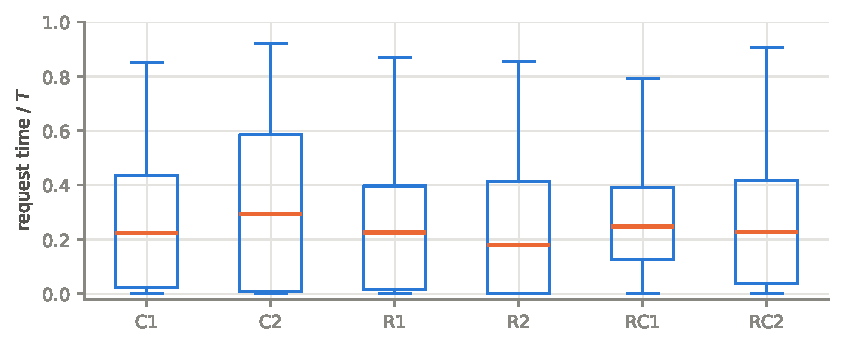
\includegraphics[width=0.85\textwidth]{figures/data_requests.pdf}
\caption{When requests arrive, as a share of the planning period $T$ (all cars of all files of each class). The box holds the middle half of the requests, the orange line is the median. About a fifth to a quarter of the requests arrive at minute 0.}
\label{fig:requests}
\end{figure}

What the table and the figure say, in words:
\begin{itemize}
  \item \textbf{The planning periods differ enormously}: R1 and RC1 have only 230--240 minutes, C2 has 3\,390. A charging session takes 27--109 minutes at a station, so in R1 and RC1 the chargers are very busy, while in C2 there is plenty of time.
  \item \textbf{Requests are spread over the whole period}, with a peak at the start (17--27\,\% at minute 0).
  \item \textbf{Every class has 15\,\% stranded cars}, which only a van can serve. With 5 vans of 6 seats there are 30 van seats; at $n=100$ about 15 of them are needed just for the stranded cars.
  \item \textbf{Stations are close}: the average car is 1--2 km from its nearest station.
\end{itemize}

\inshort{560 instances from the Solomon benchmark: six city types, short or long planning periods, 10 to 100 cars, 24 guns and 5 vans, and 15\,\% of cars that only a van can reach.}

%=====================================================================
\section{The two customer attributes: segment and income}
\label{sec:calib}

Each car carries two numbers that are written once into the dataset (\code{data/solomon\_data.csv}, columns \code{segment} and \code{theta}). The same car number has the same segment and income in every file of a class.

\subsection{Segment: 70\,\% commercial}

The model's customers are \emph{charging requests at public chargers}, not registered cars. Among electric four-wheelers registered in India in 2024 only about 10\,\% are cabs. But a cab drives about 5 times as far per day as a private car, and charges far more in public (about half of its energy, against about 10\,\% for private cars, most of whom charge at home). So a cab produces about 25 times as many public charging requests as a private car, and the share of commercial cars among requests is
\[
\pi_C=\frac{0.10\times25}{0.10\times25+0.90}=0.735,
\]
rounded down to \textbf{0.70}. In the dataset \fcomShareData\,\% of the cars are commercial.

\subsection{Income: rich private owners, lower-middle-income drivers}

\begin{itemize}
  \item \textbf{Personal cars}: about 14\,\% of urban households own a car, about 30\,\% in the richest fifth. If ownership rises with income as a power curve, the owners' income positions follow a Beta(2.5, 1) distribution (mean 0.71). Electric cars are dearer than average cars, so their owners are probably even richer; this is the least extreme choice the data allow.
  \item \textbf{Commercial cars}: surveys of app-based cab drivers report median net earnings of about Rs 15\,000 a month. That puts a driver's household around the 25th--50th income percentile: Beta(3, 5), mean 0.375. This is the least supported number and the first to replace when better data exist.
\end{itemize}

\begin{figure}[H]
\centering
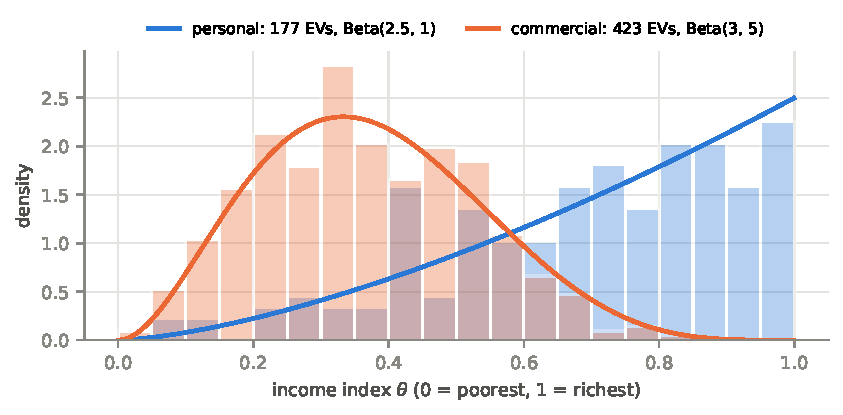
\includegraphics[width=0.85\textwidth]{figures/data_theta.pdf}
\caption{Income index of the cars in the dataset (bars: the 100 cars of each of the six classes; lines: the calibrated Beta distributions). Mean $\theta$: personal \fthetaPersData, commercial \fthetaComData. The customer population is two-humped: rich private owners and lower-middle-income drivers.}
\label{fig:theta}
\end{figure}

\inshort{Seven out of ten requests come from taxis and fleet cars, whose drivers are mostly lower-middle income; the remaining three come from mostly rich private owners.}

%=====================================================================
\section{The customer parameters}

Each sensitivity is a straight line in $\theta$, from its value at $\theta=0$ to its value at $\theta=1$, with separate end points for each segment (\code{common/f4\_params.json}).

\begin{table}[H]
\centering
\caption{End points of the customer lines. Every customer's own value is read off the line of its segment at its $\theta$.}
\small
\begin{adjustbox}{max width=\linewidth}
\begin{tabular}{@{}lrrrr@{}}
\toprule
quantity & personal $\theta=0$ & personal $\theta=1$ & commercial $\theta=0$ & commercial $\theta=1$ \\
\midrule
money sensitivity $\mu$ & 1.5 & 0.5 & 1.5 & 0.5 \\
drive to FCS $c^{D}$ (Rs/min) & 1.5 & 15 & 1.5 & 6 \\
queue at FCS $c^{Q}$ (Rs/min) & 2.5 & 25 & 2 & 7.5 \\
charge at FCS $c^{C}$ (Rs/min) & 1 & 10 & 1.5 & 6 \\
wait for / charged by van $c^{V}$ (Rs/min) & 0.5 & 5 & 1.5 & 6 \\
longest queue $W$ (min) & 60 & 15 & 40 & 15 \\
\bottomrule
\end{tabular}
\end{adjustbox}

\end{table}

\begin{figure}[H]
\centering
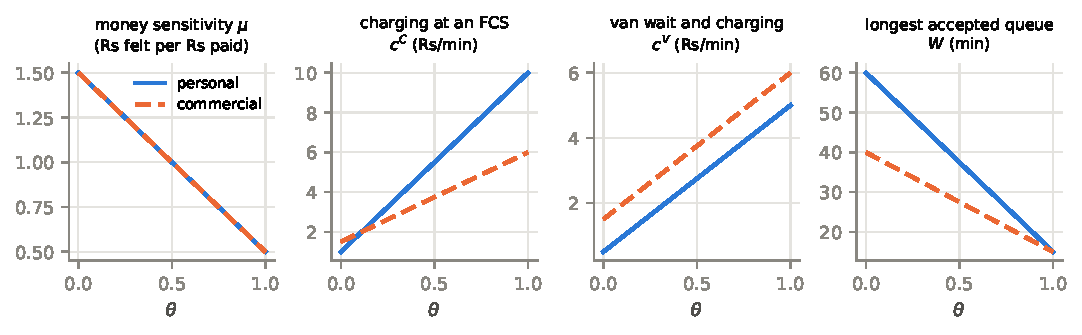
\includegraphics[width=\textwidth]{figures/data_lines.pdf}
\caption{The customer lines (blue: personal, orange dashed: commercial). Money sensitivity is the same for both segments. A personal driver's station minute gets very dear with income, while a van minute stays cheaper (driver-free). A commercial driver pays the same downtime rate for both (and it is higher than the personal van-minute value at every income).}
\label{fig:lines}
\end{figure}

How to read the lines:
\begin{itemize}
  \item \textbf{Money sensitivity $\mu$} falls from 1.5 (poorest) to 0.5 (richest), the same in both segments: a poor customer feels a rupee three times as much as a rich one.
  \item \textbf{Personal values of time} rise steeply with income: a rich owner's station minute costs Rs 10, a van minute only Rs 5 (driver free).
  \item \textbf{Commercial values of time} are one downtime rate from Rs 1.5 to Rs 6 per minute, the same for drive, station charging and van; queueing Rs 2--7.5.
  \item \textbf{Queue tolerance $W$}: 60 minutes for the poorest private owner, 40 for the poorest driver, 15 for the richest of both.
  \item \textbf{Tariffs}: Rs \fpF/kWh at a station, Rs \fpM/kWh for a van (a premium of Rs 10/kWh for charging at the door).
\end{itemize}

\inshort{Except for the segment share and income distributions, these numbers are reasoned guesses. The experiments test how much the results depend on the most important of them.}

%=====================================================================
\section{The experiments and the data each one uses}
\label{sec:experiments}

Each experiment changes \textbf{one} input and solves the same 560 instances again with both methods. Nothing else changes: same cars, same positions, same request times, same segments and incomes. No data files are copied: the solver reads \code{data/} and applies the change in memory (for example \code{--set tariff\_Rs\_per\_kWh.p\_M=35}).

\begin{table}[H]
\centering
\caption{The 15 variants of the five experiments.}
\footnotesize
\begin{adjustbox}{max width=\linewidth}
\begin{tabular}{@{}l>{\raggedright\arraybackslash}p{4.3cm}>{\raggedright\arraybackslash}p{5.6cm}>{\raggedright\arraybackslash}p{3.6cm}@{}}
\toprule
exp. & variant id & what is changed & baseline value \\
\midrule
E5 & E5\_\allowbreak cC1\_\allowbreak personal\_\allowbreak 7.5 & personal $c^{C,1}$ = 7.5 ($-$25 \%) & personal $c^{C,1}$ = 10, commercial $\omega^1$ = 6 \\
 & E5\_\allowbreak cC1\_\allowbreak personal\_\allowbreak 12.5 & personal $c^{C,1}$ = 12.5 ($+$25 \%) &  \\
 & E5\_\allowbreak omega1\_\allowbreak commercial\_\allowbreak 4.5 & commercial downtime rate at $\theta=1$: 4.5 ($-$25 \%) &  \\
 & E5\_\allowbreak omega1\_\allowbreak commercial\_\allowbreak 7.5 & commercial downtime rate at $\theta=1$: 7.5 ($+$25 \%) &  \\
\midrule
E6 & E6\_\allowbreak mu0\_\allowbreak personal\_\allowbreak 1.125 & personal $\mu^0$ = 1.125 ($-$25 \%) & personal $\mu^0$ = 1.5, commercial $\mu^0$ = 1.5 \\
 & E6\_\allowbreak mu0\_\allowbreak personal\_\allowbreak 1.875 & personal $\mu^0$ = 1.875 ($+$25 \%) &  \\
 & E6\_\allowbreak mu0\_\allowbreak commercial\_\allowbreak 1.125 & commercial $\mu^0$ = 1.125 ($-$25 \%) &  \\
 & E6\_\allowbreak mu0\_\allowbreak commercial\_\allowbreak 1.875 & commercial $\mu^0$ = 1.875 ($+$25 \%) &  \\
\midrule
E1 & E1\_\allowbreak pM\_\allowbreak 15 & $p^M$ = 15 Rs/kWh (= $p^F$) & $p^M$ = 25 \\
 & E1\_\allowbreak pM\_\allowbreak 35 & $p^M$ = 35 Rs/kWh &  \\
\midrule
E2 & E2\_\allowbreak vans\_\allowbreak 3 & 3 vans & vans = 5, seats = 6 \\
 & E2\_\allowbreak vans\_\allowbreak 7 & 7 vans &  \\
 & E2\_\allowbreak seats\_\allowbreak 4 & 4 EVs per van &  \\
 & E2\_\allowbreak seats\_\allowbreak 8 & 8 EVs per van &  \\
\midrule
E8 & E8\_\allowbreak battery\_\allowbreak 200 & B = 200 kWh & battery = 150 \\
\bottomrule
\end{tabular}
\end{adjustbox}

\end{table}

\begin{description}[leftmargin=1em]
  \item[E5 Value of charging time.] The value of a personal owner's station minute at the top income ($c^{C,1}$, the most influential guess in formulation 3), and separately the commercial downtime rate at the top income ($\omega^1$; drive, station and van minutes all change with it, queueing too). $\pm25$\,\%. \emph{Question:} how much does each segment's use of vans depend on this guess? \emph{Theory:} the personal change should move the personal van share; the commercial change should move the cost but hardly the van share.
  \item[E6 Money sensitivity.] How strongly the poorest customer feels a rupee ($\mu^0$), separately for each segment, $\pm25$\,\%. \emph{Question:} the same for the coefficient with the largest effect on $Z$. \emph{Theory:} it changes the felt cost of every tariff and drive, so $Z$ moves directly; it matters most for the segment with many poor customers (commercial).
  \item[E1 Van tariff.] $p^M$ = 15 (equal to the station price: no premium) and 35 (double premium), baseline 25. \emph{Question:} who gets vans, and what does it cost the operator and the customers? \emph{Theory:} without a premium the money reason against vans disappears, so van use rises, mostly among personal owners.
  \item[E2 Van fleet and seats.] 3 or 7 vans (baseline 5); 4 or 8 cars per van (baseline 6), one change at a time. \emph{Question:} where does another van or seat pay off?
  \item[E8 Van battery.] 200 kWh instead of 150. \emph{Question:} is van recharging worth modelling? Decision rule set in advance: if $Z$ moves by less than 1\,\%, no.
\end{description}

\textbf{How a variant is compared with the baseline.} Only on \emph{paired instances} (valid in both). For each, the change of $Z$ in \%; then the mean. The van share is pooled over all free-choice cars of the paired instances. Instances that gain or lose a valid plan are counted separately (\emph{new} and \emph{lost}).

\inshort{Five experiments, 15 variants, each changing one number; everything else, including all the data, stays the same.}

\part{The two methods}
%=====================================================================
\section{Method 1: the MILP (exact model, Gurobi)}

\subsection{What a MILP is}

A MILP writes the problem as equations. Yes/no decisions become 0/1 variables (``car 7 uses gun 3 of station 5'', ``van 2 drives from car 7 to car 12''), times become continuous variables, and every rule becomes a linear inequality (``a gun charges one car at a time'', ``the van's battery covers its route''). The software Gurobi then searches through the possible plans with \emph{branch and bound}: it solves easier versions of the problem to get a lower bound on the cost, and keeps the best plan found so far. When the best plan meets the bound, the plan is \emph{proven optimal}.

Formulation 4 has exactly the variables and the 22 rules of formulation 3 (equations (2)--(23) of \code{formulation\_4.pdf}); only each customer's cost coefficients change with segment and income. It is the \textbf{complete model}: every gun and every van is available to every car; nothing is simplified.

\subsection{How it was run}
\begin{itemize}
  \item 300 seconds per instance, 4 threads, 8 instances at a time on the 32-core server;
  \item the greedy plan (when the greedy rule finds one) is given to Gurobi as a starting point;
  \item every result is one of four: \textbf{optimal}; \textbf{time limit with a plan} (best plan found, with its gap); \textbf{time limit without a plan} (no valid plan found in 300 s); \textbf{infeasible} (proven: no plan can satisfy all rules);
  \item every plan is re-checked by an independent checker (\code{common/check\_plan\_f4.py}), which recomputes $Z$ and all rules.
\end{itemize}

\inshort{The MILP gives the best possible plan when it can prove it, a good plan with a known gap when it runs out of time, and nothing when even a first plan is too hard to find in 300 seconds.}

%=====================================================================
\section{Method 2: reinforcement learning}
\label{sec:rlmethod}

\subsection{The idea}

Instead of solving each instance from scratch, a neural network \emph{learns how to build good plans}. It is trained once, on many random instances made with the same rules as the dataset, and then builds a plan for any new instance in a fraction of a second. The method is the one of RL1 (formulation 3), rebuilt for formulation 4; it is based on the Attention Model (Kool et al.\ 2019), POMO (Kwon et al.\ 2020) and the two-step decoder of Li et al.\ (2021). The full explanation, with all papers and proofs, is in \code{RL2\_reinforcement\_learning\_method\_2/reports/RL\_implementation\_report.pdf}.

\subsection{Building a plan step by step}

The plan is built one decision at a time. Each decision is a pair: \emph{``car $i$ goes next to resource $k$''}, where $k$ is one of the 24 guns or one of the 5 vans. The car is added at the end of that gun's queue or that van's route. A \textbf{simulator} does everything that can be computed:
\begin{itemize}
  \item \textbf{times}: the session starts as early as possible (at the gun: when the car has arrived and the gun is free; with a van: when the van has arrived and the car has requested). Once the order is fixed this is always the best timing, because every time cost grows with a later start;
  \item \textbf{rules (masks)}: a pair is offered only if it breaks no rule: the station is within range, the queue is not longer than $W_i$, the car is charged by $T$; the van has a free seat, enough battery to charge this car and still get home, and is back by $T$;
  \item \textbf{cost}: the exact increase of $Z$ caused by the decision. Over a whole plan these increases add up exactly to $Z$.
\end{itemize}
If a car is left with no allowed option, it is counted as unplaced and the plan is reported as invalid.

\begin{figure}[H]
\centering
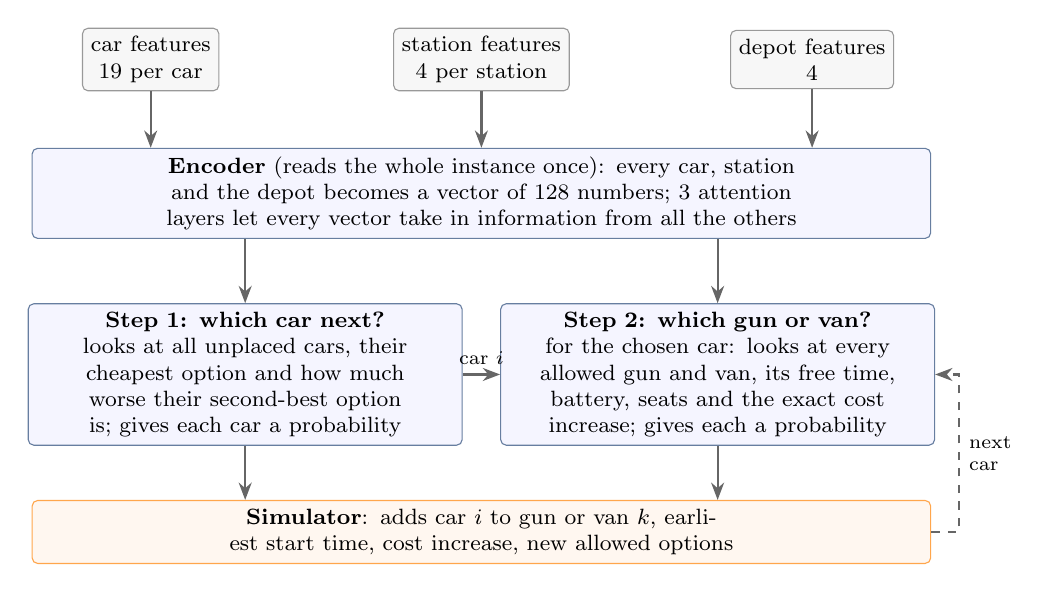
\begin{tikzpicture}[font=\footnotesize,
  box/.style={draw=headblue!70,fill=blue!4,rounded corners=2pt,align=center,minimum height=8mm,inner sep=3pt},
  data/.style={draw=black!40,fill=black!3,rounded corners=2pt,align=center,minimum height=7mm,inner sep=3pt},
  arr/.style={-{Stealth[length=2.2mm]},thick,draw=black!60}]
\node[data] (ev) at (-4.2,0) {car features\\ 19 per car};
\node[data] (st) at (0,0) {station features\\ 4 per station};
\node[data] (dep) at (4.2,0) {depot features\\ 4};
\node[box,text width=11.2cm] (enc) at (0,-1.7) {\textbf{Encoder} (reads the whole instance once): every car, station and the depot becomes a vector of 128 numbers; 3 attention layers let every vector take in information from all the others};
\draw[arr] (ev) -- (ev |- enc.north);
\draw[arr] (st) -- (enc);
\draw[arr] (dep) -- (dep |- enc.north);
\node[box,text width=5.3cm] (d1) at (-3.0,-4.0) {\textbf{Step 1: which car next?}\\ looks at all unplaced cars, their cheapest option and how much worse their second-best option is; gives each car a probability};
\node[box,text width=5.3cm] (d2) at (3.0,-4.0) {\textbf{Step 2: which gun or van?}\\ for the chosen car: looks at every allowed gun and van, its free time, battery, seats and the exact cost increase; gives each a probability};
\draw[arr] (enc.south -| d1) -- (d1.north);
\draw[arr] (enc.south -| d2) -- (d2.north);
\draw[arr] (d1.east) -- node[above,font=\scriptsize]{car $i$} (d2.west);
\node[box,text width=11.2cm,fill=orange!6,draw=orange!70] (env) at (0,-6.0) {\textbf{Simulator}: adds car $i$ to gun or van $k$, earliest start time, cost increase, new allowed options};
\draw[arr] (d1) -- (d1 |- env.north);
\draw[arr] (d2) -- (d2 |- env.north);
\draw[arr,dashed] (env.east) -- ++(0.35,0) |- node[pos=0.25,right,font=\scriptsize,align=left]{next\\ car} (d2.east);
\end{tikzpicture}
\caption{The RL policy. The encoder runs once per instance; steps 1 and 2 and the simulator run once for every car placed.}
\label{fig:arch}
\end{figure}

\subsection{The network (architecture)}

\begin{itemize}
  \item \textbf{Inputs.} Each car is described by 19 numbers: its position, request time, charging times at a station and by a van, energy, queue tolerance, income, whether it is stranded, how many stations it can reach and how far the nearest is, how far it is from the depot, its cheapest station option and van option, how late a van may come, and three numbers new in formulation 4: \emph{commercial or not}, its money sensitivity $\mu$, and the cost of queueing for one charging duration ($c^Q\tau^F$). Each station has 4 numbers (position, guns, share of cars that can reach it), the depot 4 (seats per car, guns per car, length of the period, size). All numbers are scaled (by $T$, the battery, the city size or the instance's typical cost) so that small and large, short and long instances look alike to the network.
  \item \textbf{Encoder.} A Transformer of 3 layers, 8 attention heads, vectors of 128 numbers. Attention is a weighted average: each car's vector is updated with a mix of all other vectors, with weights the network learns. There is no fixed order of the cars, so the same network works for 10 or 100 cars.
  \item \textbf{Decoder, step 1 (which car).} Combines the average of the unplaced cars, the depot and 4 numbers about the progress of the plan; scores every unplaced car using its vector plus 7 numbers that change during the construction (options left, cheapest option, regret = second-cheapest minus cheapest, earliest finish, gun versus van cost, how soon it requested, its place in the queue of open requests).
  \item \textbf{Decoder, step 2 (which resource).} For the chosen car, scores every gun (by its station's vector) and every van (by the vector of the place where it now is), plus each resource's state and 6 numbers about the exact pair (its cost increase, its wait, finish, battery left after it).
  \item \textbf{Size.} \frlParams{} learned weights.
\end{itemize}

\subsection{How it learns}
\begin{enumerate}
  \item \textbf{Random training instances} are drawn with the dataset's rules: new positions (clustered, random or mixed), stations by $k$-means, energies, ranges with 15\,\% stranded, request times, and \emph{segment} (70\,\% commercial) and \emph{income} from the calibrated distributions. The 56 test files are never used in training.
  \item \textbf{Warm-up by imitation} (first 500 batches): the network learns to copy the greedy rule (stranded cars first, then by request time, then the cars that hate queueing most; each takes its cheapest allowed option). This gives a sensible start instead of random behaviour.
  \item \textbf{Reinforcement learning} (REINFORCE with a shared baseline): every training instance is solved 8 times by sampling; the plans cheaper than the average of the 8 are made more likely, the dearer ones less likely. 32 instances per batch, 50 batches per epoch.
  \item \textbf{Stopping}: at least 200 epochs; then stop after 10 epochs without a better result on fixed validation instances, at most 500 epochs. The network of the best epoch is kept.
\end{enumerate}

\begin{figure}[H]
\centering
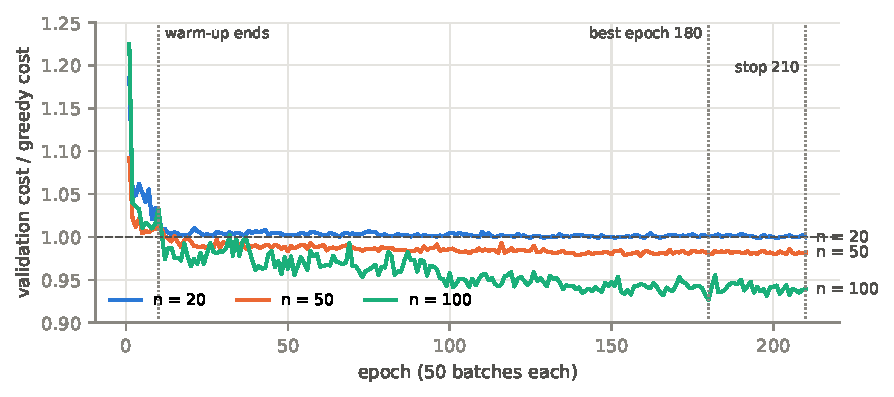
\includegraphics[width=0.88\textwidth]{figures/rl_training.pdf}
\caption{Training of the baseline RL policy: cost of its plans divided by the greedy rule's cost on fixed validation instances (below 1 = better than greedy). Untrained it costs \frlUntrained{} times the greedy rule; after one warm-up epoch \frlAfterWarmOne{}. Best at epoch \frlBestEpoch{} (\frlBestVal); stopped at epoch \frlStopEpoch{} after \frlTrainMin{} minutes on the RTX 4090. The gain over greedy is largest for large instances.}
\label{fig:rltrain}
\end{figure}

\subsection{How it solves a test instance}

The map is turned and mirrored in 8 ways (distances stay the same, but the network sees different coordinates). For each, the policy builds 1 plan taking always its most likely choice and 64 plans by sampling: 520 plans in all. The plan with the fewest unplaced cars, then the lowest $Z$, is kept and scored by the same checker as the MILP.

\subsection{Zero-shot and retrained runs in the experiments}

For each experiment variant RL gives two runs:
\begin{itemize}
  \item \textbf{zero-shot}: the baseline policy, unchanged, applied to the changed data. This works because the network's inputs contain the changed numbers (tariffs and costs through the cost increases, $\mu$, the fleet). It tests whether one trained policy can be reused when an assumption changes;
  \item \textbf{retrained}: a new policy trained from scratch with the variant's values, same recipe (about 39 minutes each, 15 models).
\end{itemize}

\inshort{The RL policy builds a plan car by car, choosing first a car and then a gun or van; a simulator keeps every step legal and exactly costed. It learns once from random examples and then solves any instance in about a tenth of a second.}

\part{Results of the MILP}
%=====================================================================
\section{MILP baseline: how the 560 instances ended}

\begin{figure}[H]
\centering
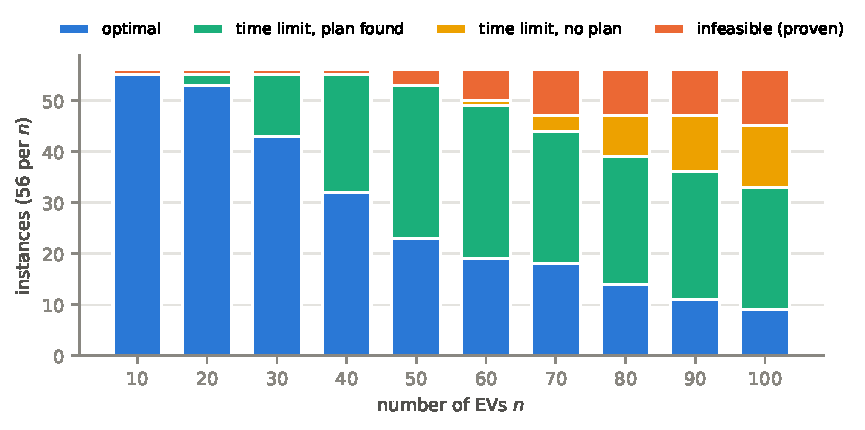
\includegraphics[width=0.88\textwidth]{figures/milp_status_by_n.pdf}
\caption{Result of the MILP for each instance size (56 instances per size).}
\label{fig:status}
\end{figure}

\begin{table}[H]
\centering
\caption{MILP baseline by Solomon class. Median gap: over the time-limited instances with a plan.}
\small
\begin{adjustbox}{max width=\linewidth}
\begin{tabular}{@{}lrrrrrrrrr@{}}
\toprule
class & instances & optimal & time limit & no plan & infeasible & valid & \shortstack{median\\gap (\%)} & \shortstack{mean\\time (s)} & \shortstack{mean $Z$\\(Rs)} \\
\midrule
C1 & 90 & 66 & 23 & 1 & 0 & 89 & 4.1 & 110 & 47470 \\
C2 & 80 & 56 & 23 & 1 & 0 & 79 & 2.9 & 109 & 47996 \\
R1 & 120 & 41 & 34 & 16 & 29 & 75 & 4.4 & 137 & 32677 \\
R2 & 110 & 70 & 40 & 0 & 0 & 110 & 2.6 & 130 & 44782 \\
RC1 & 80 & 13 & 29 & 16 & 22 & 42 & 7.8 & 171 & 36587 \\
RC2 & 80 & 31 & 48 & 1 & 0 & 79 & 2.9 & 189 & 49691 \\
\bottomrule
\end{tabular}
\end{adjustbox}

\end{table}

\begin{itemize}
  \item \textbf{\fmilpOptimal{} instances optimal}, \fmilpTL{} stopped at the time limit with a plan (median gap \fmilpGapMedian\,\%, mean \fmilpGapMean\,\%), \fmilpTLnoPlan{} stopped \emph{without} a plan, \fmilpInfeasible{} proven infeasible. In total \fmilpValid{} valid plans. Mean solve time \fmilpSolveMean{} s.
  \item \textbf{Size decides difficulty.} Up to 20 cars almost everything is optimal in seconds. From about 50 cars, most instances hit the 300-second limit.
  \item \textbf{The infeasible and unsolved instances are in R1 and RC1}, the classes with very short periods (230--240 min). There 100 cars, many requesting late, cannot all be charged by $T$ with 24 guns and 5 vans. The 51 infeasible instances are exactly the 51 of formulation 3: infeasibility comes from the data (time, range, fleet), not from the customer numbers.
  \item The greedy rule alone finds a valid plan in \fgreedyValid{} instances; the MILP starts from that plan and finds valid plans in 13 more instances.
  \item Compared with formulation 3 (same data, one customer type), formulation 4 proves more instances optimal (277 against 256); the other statuses are almost unchanged.
\end{itemize}

\inshort{The MILP solves small instances to optimality and large ones to within a few per cent; the only failures are the short-period classes R1 and RC1 at 60--100 cars, mostly because no plan can exist there.}

%=====================================================================
\section{MILP baseline: what the cost is made of}
\label{sec:anatomy}

\begin{table}[H]
\centering
\caption{The six parts of $Z$, over the \fmilpValid{} valid MILP plans.}
\small
\begin{adjustbox}{max width=\linewidth}
\begin{tabular}{@{}lrr@{}}
\toprule
term & mean per instance (Rs) & share of $Z$ (\%) \\
\midrule
$Z_1$ EV driving (perceived) & 388 & 0.9 \\
$Z_2$ van driving & 1067 & 2.4 \\
$Z_3$ van dispatch & 3291 & 7.5 \\
$Z_4$ operator energy & 9204 & 20.9 \\
$Z_5$ tariff (perceived) & 17310 & 39.3 \\
$Z_6$ time (perceived) & 12739 & 29.0 \\
\midrule
$Z$ (all six) & 43999 & 100.0 \\
\bottomrule
\end{tabular}
\end{adjustbox}

\end{table}

\begin{itemize}
  \item \textbf{The tariff felt by customers ($Z_5$) is the largest part} (\fshareZFive\,\%): every car pays for 10--40 kWh, and most customers are poor commercial drivers who feel each rupee strongly.
  \item \textbf{Customers' time ($Z_6$) is next} (\fshareZSix\,\%): about an hour per car from request to full charge.
  \item \textbf{The operator's energy ($Z_4$)} is \fshareZFour\,\%; van dispatch \fshareZThree\,\%; van driving and EV driving are small.
\end{itemize}

\inshort{Two thirds of $Z$ is what customers feel (money and time); a third is the operator's cost, mostly electricity.}

%=====================================================================
\section{MILP baseline: who gets a van}

\begin{table}[H]
\centering
\caption{The two segments in the baseline plans of the MILP and of RL (RL is discussed in Part V). Free-choice cars have a station within range. Note: the MILP and RL columns are over their own valid plans (\fmilpValid{} and \frlValid{} instances).}
\small
\begin{adjustbox}{max width=\linewidth}
\begin{tabular}{@{}lrrrr@{}}
\toprule
 & personal MILP & personal RL & commercial MILP & commercial RL \\
\midrule
EVs in valid plans & 7043 & 7768 & 16787 & 18282 \\
free-choice EVs & 6095 & 6727 & 14125 & 15418 \\
van share of free-choice EVs (\%) & 19.9 & 6.7 & 0.7 & 0.9 \\
mean $\theta$ & 0.69 & 0.69 & 0.36 & 0.36 \\
mean queue at FCS (min) & 0.41 & 0.79 & 1.58 & 3.36 \\
mean wait for a van (min) & 19.8 & 21.8 & 24.5 & 28.3 \\
mean drive to FCS (min) & 7.8 & 8.3 & 8.9 & 11.3 \\
mean time until charged (min) & 60.6 & 61.8 & 64.3 & 68.3 \\
mean money paid (Rs) & 352 & 332 & 335 & 337 \\
mean time cost (Rs) & 381 & 430 & 200 & 214 \\
mean perceived cost (Rs) & 662 & 699 & 582 & 597 \\
\bottomrule
\end{tabular}
\end{adjustbox}

\end{table}

\begin{figure}[H]
\centering
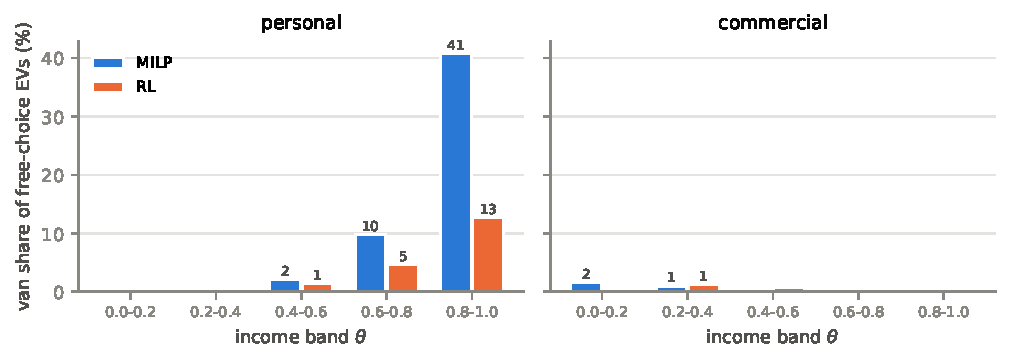
\includegraphics[width=0.95\textwidth]{figures/van_share_income.pdf}
\caption{Share of free-choice cars served by a van, by segment and income band (numbers above the bars in \%).}
\label{fig:vanincome}
\end{figure}

\begin{table}[H]
\centering
\caption{By income band (MILP, all valid plans; van share also for RL). ``Money felt'' is the money paid times the customer's $\mu$.}
\footnotesize
\begin{adjustbox}{max width=\linewidth}
\begin{tabular}{@{}llrrrrrrr@{}}
\toprule
segment & \shortstack{$\theta$\\band} & EVs & van \% MILP & van \% RL & queue (min) & \shortstack{money\\felt (Rs)} & \shortstack{time cost\\(Rs)} & \shortstack{perceived\\cost (Rs)} \\
\midrule
personal & 0.0-0.2 & 125 & 0.0 & 0.0 & 1.45 & 389 & 120 & 509 \\
 & 0.2-0.4 & 690 & 0.0 & 0.0 & 1.32 & 403 & 243 & 646 \\
 & 0.4-0.6 & 1491 & 2.1 & 1.4 & 0.57 & 338 & 337 & 675 \\
 & 0.6-0.8 & 1934 & 9.8 & 4.7 & 0.18 & 263 & 428 & 691 \\
 & 0.8-1.0 & 2803 & 40.8 & 12.7 & 0.06 & 228 & 418 & 646 \\
\midrule
commercial & 0.0-0.2 & 2532 & 1.6 & 0.5 & 2.77 & 457 & 151 & 607 \\
 & 0.2-0.4 & 7633 & 1.0 & 1.3 & 1.76 & 408 & 186 & 594 \\
 & 0.4-0.6 & 5356 & 0.1 & 0.7 & 0.92 & 333 & 226 & 560 \\
 & 0.6-0.8 & 1186 & 0.0 & 0.5 & 0.75 & 286 & 273 & 559 \\
 & 0.8-1.0 & 80 & 0.0 & 0.0 & 0.00 & 167 & 258 & 425 \\
\bottomrule
\end{tabular}
\end{adjustbox}

\end{table}

What the MILP plans show:
\begin{enumerate}
  \item \textbf{Vans go to personal cars.} \fvanPersMilp\,\% of free-choice personal cars get a van, against \fvanComMilp\,\% of commercial cars. This is theory point 3: the driver-free benefit belongs to private owners.
  \item \textbf{Among personal cars, van use rises steeply with income}: 0\,\% below $\theta=0.4$, 2\,\% at 0.4--0.6, 10\,\% at 0.6--0.8, 41\,\% above 0.8. A logistic fit of ``van or not'' on $\theta$ puts the income threshold for personal cars at $\theta^*\approx\fthetaStarPers$: only the very richest are more likely than not to get a van. For commercial cars there is no threshold in $[0,1]$.
  \item \textbf{The few commercial cars with a van are the poorest drivers}, not the richest (1.6\,\% below $\theta=0.2$, 0\,\% above 0.6). They are also the ones with the longest station queues (2.8 minutes on average in the lowest band, 0 in the highest). This is theory point 2: \emph{queues, not income, push taxis to vans}.
  \item \textbf{Commercial cars wait more at stations} (\fqueueComMilp{} against \fqueuePersMilp{} minutes on average) and take longer until charged (64 against 61 minutes). Low-income customers absorb the queues, as theory point 5 predicts.
  \item \textbf{Money paid is about the same in both segments} (about Rs 335--350), but \textbf{money felt} is much higher for commercial drivers (Rs 382 against 281), because they are poorer. Personal owners instead lose more in \emph{time} value (Rs 381 against 200).
  \item By class, the personal van share is lowest in R1 (12\,\%: very short period, a van can make few trips) and highest in RC2 (26\,\%).
\end{enumerate}

\inshort{In the best plans, vans are a service for rich private owners; taxis and poorer customers use the stations and absorb the queues. The rare taxi with a van is a poor driver escaping a long queue.}

%=====================================================================
\section{MILP experiments, one by one}
\label{sec:milpexp}

Each table below shows the MILP row first and then the two RL rows (discussed in Part V). Columns: valid plans; paired instances; instances \emph{new}ly valid or \emph{lost} against the baseline; mean change of $Z$, of the operator's cost and of the customers' cost (paired instances); van share of free-choice cars, baseline $\to$ variant; average number of vans used; for RL the mean gap to the MILP of the same variant.

\subsection{E5: value of charging time}

\begin{table}[H]
\centering
\caption{E5. Value of a station minute for the richest private owner ($c^{C,1}$), and the commercial downtime rate at the top income ($\omega^1$), $\pm25$\,\%.}
\scriptsize
\begin{adjustbox}{max width=\linewidth}
\begin{tabular}{@{}lrrrrrrrrrrr@{}}
\toprule
method & valid & paired & new & lost & \shortstack{$\Delta Z$\\\%} & \shortstack{$\Delta$\\oper. \%} & \shortstack{$\Delta$\\cust. \%} & \shortstack{van \%\\personal} & van \% comm. & vans used & \shortstack{gap to\\MILP \%} \\
\midrule
\multicolumn{12}{@{}l}{\textbf{E5\_cC1\_personal\_7.5}: personal $c^{C,1}$ = 7.5 ($-$25 \%)} \\
MILP & 473 & 472 & 1 & 2 & $-$2.21 & $-$1.15 & $-$2.59 & 19.9 $\to$ 14.1 & 0.7 $\to$ 0.8 & 2.13 & -- \\
RL zero-shot & 499 & 499 & 0 & 1 & $-$2.49 & $-$0.21 & $-$3.45 & 6.7 $\to$ 5.5 & 0.9 $\to$ 0.9 & 2.20 & 0.56 \\
RL retrained & 500 & 499 & 1 & 1 & $-$2.46 & $-$0.59 & $-$3.24 & 6.7 $\to$ 3.9 & 0.9 $\to$ 0.8 & 2.19 & 0.56 \\
\multicolumn{12}{@{}l}{\textbf{E5\_cC1\_personal\_12.5}: personal $c^{C,1}$ = 12.5 ($+$25 \%)} \\
MILP & 473 & 472 & 1 & 2 & $+$2.08 & $+$2.75 & $+$1.84 & 19.9 $\to$ 29.4 & 0.7 $\to$ 0.7 & 2.37 & -- \\
RL zero-shot & 502 & 500 & 2 & 0 & $+$2.45 & $+$0.32 & $+$3.37 & 6.7 $\to$ 8.0 & 0.9 $\to$ 0.8 & 2.23 & 1.22 \\
RL retrained & 500 & 500 & 0 & 0 & $+$2.38 & $+$0.93 & $+$3.02 & 6.7 $\to$ 11.7 & 0.9 $\to$ 0.6 & 2.26 & 1.14 \\
\multicolumn{12}{@{}l}{\textbf{E5\_omega1\_commercial\_4.5}: commercial downtime rate at $\theta=1$: 4.5 ($-$25 \%)} \\
MILP & 472 & 471 & 1 & 3 & $-$2.67 & $-$0.17 & $-$3.80 & 19.9 $\to$ 19.6 & 0.7 $\to$ 0.7 & 2.17 & -- \\
RL zero-shot & 500 & 499 & 1 & 1 & $-$2.72 & $-$0.13 & $-$3.86 & 6.7 $\to$ 6.5 & 0.9 $\to$ 0.8 & 2.19 & 0.82 \\
RL retrained & 500 & 499 & 1 & 1 & $-$2.52 & $+$0.17 & $-$3.69 & 6.7 $\to$ 7.6 & 0.9 $\to$ 0.6 & 2.23 & 0.98 \\
\multicolumn{12}{@{}l}{\textbf{E5\_omega1\_commercial\_7.5}: commercial downtime rate at $\theta=1$: 7.5 ($+$25 \%)} \\
MILP & 475 & 472 & 3 & 2 & $+$2.66 & $+$0.26 & $+$3.81 & 19.9 $\to$ 19.6 & 0.7 $\to$ 0.7 & 2.20 & -- \\
RL zero-shot & 500 & 500 & 0 & 0 & $+$2.72 & $+$0.26 & $+$3.82 & 6.7 $\to$ 6.9 & 0.9 $\to$ 0.9 & 2.24 & 0.83 \\
RL retrained & 499 & 499 & 0 & 1 & $+$2.75 & $+$0.14 & $+$3.92 & 6.7 $\to$ 7.0 & 0.9 $\to$ 0.8 & 2.22 & 0.86 \\
\bottomrule
\end{tabular}
\end{adjustbox}

\end{table}

\begin{itemize}
  \item \textbf{Personal $c^{C,1}$} moves $Z$ by $-2.2$\,\% / $+2.1$\,\% and \textbf{strongly moves the personal van share}: 19.9\,\% $\to$ 14.1\,\% when station time is valued less, $\to$ 29.4\,\% when it is valued more. When rich owners hate station time more, more of them get vans, and the operator pays for it (operator cost $+2.75$\,\%).
  \item \textbf{Commercial $\omega^1$} moves $Z$ by $\mp2.7$\,\% but \textbf{does not change who gets vans} (personal 19.6\,\%, commercial 0.7\,\% in both variants). A taxi's drive, charge and van minutes all scale with $\omega$, so both options become dearer together; only the customers' cost changes ($\pm3.8$\,\%).
  \item Both results are what theory predicted for E5.
\end{itemize}

\inshort{How much private owners hate station time decides how many vans they get; the taxi downtime rate changes the cost but not the choices.}

\subsection{E6: money sensitivity}

\begin{table}[H]
\centering
\caption{E6. How strongly the poorest customer feels a rupee ($\mu^0$), per segment, $\pm25$\,\%.}
\scriptsize
\begin{adjustbox}{max width=\linewidth}
\begin{tabular}{@{}lrrrrrrrrrrr@{}}
\toprule
method & valid & paired & new & lost & \shortstack{$\Delta Z$\\\%} & \shortstack{$\Delta$\\oper. \%} & \shortstack{$\Delta$\\cust. \%} & \shortstack{van \%\\personal} & van \% comm. & vans used & \shortstack{gap to\\MILP \%} \\
\midrule
\multicolumn{12}{@{}l}{\textbf{E6\_mu0\_personal\_1.125}: personal $\mu^0$ = 1.125 ($-$25 \%)} \\
MILP & 473 & 472 & 1 & 2 & $-$1.35 & $-$0.01 & $-$1.96 & 19.9 $\to$ 19.8 & 0.7 $\to$ 0.6 & 2.18 & -- \\
RL zero-shot & 500 & 499 & 1 & 1 & $-$1.28 & $+$0.10 & $-$1.89 & 6.7 $\to$ 7.0 & 0.9 $\to$ 0.9 & 2.21 & 0.92 \\
RL retrained & 501 & 500 & 1 & 0 & $-$1.22 & $+$0.07 & $-$1.79 & 6.7 $\to$ 7.8 & 0.9 $\to$ 0.7 & 2.21 & 0.95 \\
\multicolumn{12}{@{}l}{\textbf{E6\_mu0\_personal\_1.875}: personal $\mu^0$ = 1.875 ($+$25 \%)} \\
MILP & 475 & 473 & 2 & 1 & $+$1.33 & $-$0.15 & $+$2.04 & 19.9 $\to$ 18.9 & 0.7 $\to$ 0.7 & 2.18 & -- \\
RL zero-shot & 500 & 499 & 1 & 1 & $+$1.29 & $-$0.03 & $+$1.89 & 6.7 $\to$ 6.5 & 0.9 $\to$ 0.8 & 2.21 & 0.80 \\
RL retrained & 499 & 499 & 0 & 1 & $+$1.36 & $+$0.10 & $+$1.94 & 6.7 $\to$ 7.3 & 0.9 $\to$ 0.8 & 2.22 & 0.84 \\
\multicolumn{12}{@{}l}{\textbf{E6\_mu0\_commercial\_1.125}: commercial $\mu^0$ = 1.125 ($-$25 \%)} \\
MILP & 475 & 474 & 1 & 0 & $-$6.38 & $+$0.05 & $-$9.40 & 19.9 $\to$ 19.6 & 0.7 $\to$ 0.7 & 2.20 & -- \\
RL zero-shot & 499 & 499 & 0 & 1 & $-$6.31 & $+$0.07 & $-$9.18 & 6.7 $\to$ 6.8 & 0.9 $\to$ 0.9 & 2.21 & 0.87 \\
RL retrained & 500 & 500 & 0 & 0 & $-$6.25 & $-$0.12 & $-$9.01 & 6.7 $\to$ 7.1 & 0.9 $\to$ 0.8 & 2.19 & 0.91 \\
\multicolumn{12}{@{}l}{\textbf{E6\_mu0\_commercial\_1.875}: commercial $\mu^0$ = 1.875 ($+$25 \%)} \\
MILP & 475 & 473 & 2 & 1 & $+$6.43 & $+$0.06 & $+$9.47 & 19.9 $\to$ 19.8 & 0.7 $\to$ 0.7 & 2.19 & -- \\
RL zero-shot & 500 & 499 & 1 & 1 & $+$6.34 & $+$0.04 & $+$9.19 & 6.7 $\to$ 6.8 & 0.9 $\to$ 0.9 & 2.21 & 0.80 \\
RL retrained & 500 & 499 & 1 & 1 & $+$6.33 & $+$0.12 & $+$9.15 & 6.7 $\to$ 7.8 & 0.9 $\to$ 0.6 & 2.21 & 0.79 \\
\bottomrule
\end{tabular}
\end{adjustbox}

\end{table}

\begin{itemize}
  \item \textbf{Commercial $\mu^0$ is the strongest lever of all experiments}: $Z$ $-6.4$\,\% / $+6.4$\,\%, almost all on the customers' side ($\mp9.4$\,\%). Commercial drivers are 70\,\% of the customers and mostly poor, so their $\mu$ is close to $\mu^0$; every rupee they pay for tariffs and driving is weighted by it, and the tariff is the largest part of $Z$.
  \item \textbf{Personal $\mu^0$ matters much less} ($\pm1.3$\,\%): private owners are rich, their $\mu$ is close to $\mu^1=0.5$, which does not change.
  \item \textbf{Nobody changes resource}: van shares stay at about 19--20\,\% and 0.6--0.7\,\%. A larger $\mu$ makes the station and the van dearer in the same proportion (both tariffs are multiplied by $\mu$); only the van premium becomes a little more painful.
\end{itemize}

\inshort{How poor drivers feel money is the assumption $Z$ depends on most, but it changes the size of the cost, not the plan.}

\subsection{E1: van tariff}

\begin{table}[H]
\centering
\caption{E1. Van tariff $p^M$ = 15 (no premium) and 35 Rs/kWh (baseline 25).}
\scriptsize
\begin{adjustbox}{max width=\linewidth}
\begin{tabular}{@{}lrrrrrrrrrrr@{}}
\toprule
method & valid & paired & new & lost & \shortstack{$\Delta Z$\\\%} & \shortstack{$\Delta$\\oper. \%} & \shortstack{$\Delta$\\cust. \%} & \shortstack{van \%\\personal} & van \% comm. & vans used & \shortstack{gap to\\MILP \%} \\
\midrule
\multicolumn{12}{@{}l}{\textbf{E1\_pM\_15}: $p^M$ = 15 Rs/kWh (= $p^F$)} \\
MILP & 471 & 470 & 1 & 4 & $-$4.19 & $+$3.69 & $-$7.80 & 19.8 $\to$ 31.4 & 0.7 $\to$ 1.4 & 2.40 & -- \\
RL zero-shot & 500 & 499 & 1 & 1 & $-$3.74 & $+$0.45 & $-$5.66 & 6.7 $\to$ 8.4 & 0.9 $\to$ 1.0 & 2.22 & 1.31 \\
RL retrained & 499 & 499 & 0 & 1 & $-$3.78 & $+$1.04 & $-$5.97 & 6.7 $\to$ 11.3 & 0.9 $\to$ 1.0 & 2.26 & 1.25 \\
\multicolumn{12}{@{}l}{\textbf{E1\_pM\_35}: $p^M$ = 35 Rs/kWh} \\
MILP & 477 & 474 & 3 & 0 & $+$3.91 & $-$1.39 & $+$6.53 & 19.9 $\to$ 13.5 & 0.7 $\to$ 0.8 & 2.12 & -- \\
RL zero-shot & 499 & 498 & 1 & 2 & $+$3.64 & $-$0.36 & $+$5.49 & 6.7 $\to$ 5.1 & 0.9 $\to$ 0.8 & 2.18 & 0.58 \\
RL retrained & 500 & 499 & 1 & 1 & $+$3.73 & $-$0.76 & $+$5.80 & 6.7 $\to$ 1.1 & 0.9 $\to$ 0.9 & 2.18 & 0.64 \\
\bottomrule
\end{tabular}
\end{adjustbox}

\end{table}

\begin{figure}[H]
\centering
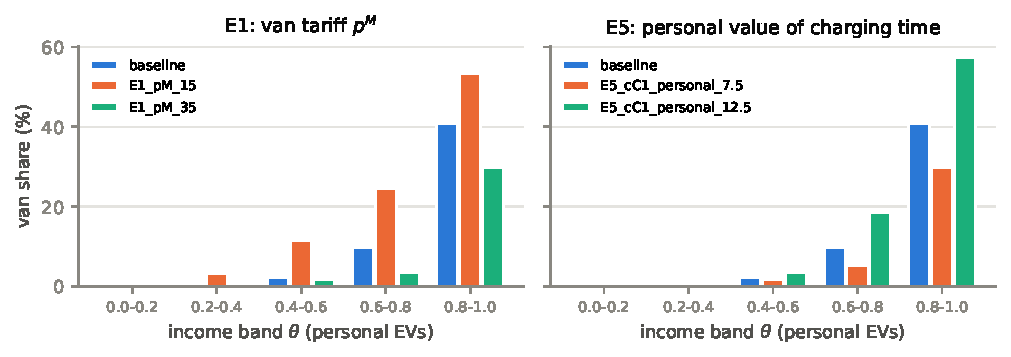
\includegraphics[width=0.95\textwidth]{figures/exp_income.pdf}
\caption{Personal van share by income band (MILP): E1 (van tariff) and E5 (personal value of charging time).}
\label{fig:expincome}
\end{figure}

\begin{itemize}
  \item \textbf{No premium ($p^M=15$)}: $Z$ $-4.2$\,\%. Customers save 7.8\,\%, the operator pays 3.7\,\% more (more vans dispatched, 2.40 instead of 2.17 on average, and dearer van energy). Personal van share 19.8\,\% $\to$ 31.4\,\%; van use spreads down the income scale (Figure~\ref{fig:expincome}: 0.4--0.6 band from 2\,\% to 12\,\%, 0.6--0.8 from 10\,\% to 24\,\%). Commercial van share doubles but stays small (0.7 $\to$ 1.4\,\%).
  \item \textbf{Double premium ($p^M=35$)}: $Z$ $+3.9$\,\%, customers $+6.5$\,\%, operator $-1.4$\,\%. Personal van share falls to 13.5\,\%; even the richest band drops from 41\,\% to 30\,\%.
  \item \textbf{Who gains from cheaper vans}: mostly rich private owners (their felt cost in the top band falls from about Rs 646 to 547), because they are the ones who switch. Poor drivers gain little (Rs 607 to 576), mostly because the stations get less crowded.
  \item 4 instances lose their plan at $p^M=15$ and 3 gain one at $p^M=35$: with more van use the 300-second search gets harder, not the problem itself.
\end{itemize}

\inshort{The van price is the operator's main tool to decide how many and which customers get vans; making vans cheaper mostly helps rich private owners.}

\subsection{E2: van fleet and seats}

\begin{table}[H]
\centering
\caption{E2. 3 or 7 vans (baseline 5); 4 or 8 cars per van (baseline 6).}
\scriptsize
\begin{adjustbox}{max width=\linewidth}
\begin{tabular}{@{}lrrrrrrrrrrr@{}}
\toprule
method & valid & paired & new & lost & \shortstack{$\Delta Z$\\\%} & \shortstack{$\Delta$\\oper. \%} & \shortstack{$\Delta$\\cust. \%} & \shortstack{van \%\\personal} & van \% comm. & vans used & \shortstack{gap to\\MILP \%} \\
\midrule
\multicolumn{12}{@{}l}{\textbf{E2\_vans\_3}: 3 vans} \\
MILP & 441 & 441 & 0 & 33 & $-$0.04 & $-$0.53 & $+$0.20 & 19.4 $\to$ 17.4 & 0.2 $\to$ 0.1 & 1.96 & -- \\
RL zero-shot & 465 & 465 & 0 & 35 & $+$0.02 & $-$0.27 & $+$0.15 & 6.4 $\to$ 5.7 & 0.3 $\to$ 0.2 & 2.00 & 0.91 \\
RL retrained & 466 & 466 & 0 & 34 & $+$0.09 & $-$0.12 & $+$0.18 & 6.4 $\to$ 5.9 & 0.4 $\to$ 0.2 & 2.02 & 0.96 \\
\multicolumn{12}{@{}l}{\textbf{E2\_vans\_7}: 7 vans} \\
MILP & 487 & 474 & 13 & 0 & $+$0.02 & $+$0.22 & $-$0.05 & 19.9 $\to$ 20.5 & 0.7 $\to$ 0.7 & 2.22 & -- \\
RL zero-shot & 506 & 500 & 6 & 0 & $+$0.04 & $+$0.13 & $+$0.03 & 6.7 $\to$ 6.7 & 0.9 $\to$ 1.0 & 2.23 & 0.84 \\
RL retrained & 506 & 500 & 6 & 0 & $+$0.00 & $+$0.06 & $-$0.00 & 6.7 $\to$ 7.0 & 0.9 $\to$ 0.7 & 2.23 & 0.81 \\
\multicolumn{12}{@{}l}{\textbf{E2\_seats\_4}: 4 EVs per van} \\
MILP & 471 & 467 & 4 & 7 & $+$1.08 & $+$3.03 & $+$0.26 & 19.8 $\to$ 11.6 & 0.3 $\to$ 0.2 & 2.48 & -- \\
RL zero-shot & 493 & 493 & 0 & 7 & $+$0.91 & $+$3.87 & $-$0.35 & 6.7 $\to$ 5.8 & 0.5 $\to$ 0.4 & 2.54 & 0.69 \\
RL retrained & 494 & 494 & 0 & 6 & $+$0.88 & $+$4.04 & $-$0.46 & 6.8 $\to$ 7.2 & 0.5 $\to$ 0.3 & 2.55 & 0.65 \\
\multicolumn{12}{@{}l}{\textbf{E2\_seats\_8}: 8 EVs per van} \\
MILP & 471 & 471 & 0 & 3 & $-$0.08 & $-$0.28 & $+$0.06 & 19.9 $\to$ 21.6 & 0.7 $\to$ 0.8 & 2.13 & -- \\
RL zero-shot & 500 & 499 & 1 & 1 & $-$0.08 & $-$0.61 & $+$0.16 & 6.7 $\to$ 6.6 & 0.9 $\to$ 0.9 & 2.13 & 0.85 \\
RL retrained & 499 & 499 & 0 & 1 & $+$0.07 & $-$0.31 & $+$0.25 & 6.7 $\to$ 7.2 & 0.9 $\to$ 0.9 & 2.16 & 0.98 \\
\bottomrule
\end{tabular}
\end{adjustbox}

\end{table}

\begin{itemize}
  \item \textbf{The number of vans does not change the cost} of solvable instances: on the instances optimal in both runs the change is 0.000\,\% for 3 and for 7 vans (Table~\ref{tab:direction}). The plans use only about 2.2 vans on average, so the fifth van is rarely needed for cost.
  \item \textbf{But the number of vans decides feasibility}: with 3 vans 33 instances lose their plan (3 become provably infeasible), with 7 vans 13 new instances get one. These are mostly large R1/RC1 instances (23 of the 33 lost, 10 of the 13 gained; all with 50 or more cars), where stranded cars and late requests need many van trips in a short period. The small changes in the table ($-0.04$\,\%, $+0.02$\,\%) come from time-limited plans, not from a real effect.
  \item \textbf{Fewer seats per van cost money}: with 4 seats $Z$ rises 1.1\,\% (1.3\,\% at the optima), the operator's cost 3.0\,\%: more vans must be dispatched (2.48 instead of about 2.2) to serve the same cars, and the personal van share falls from 19.8 to 11.6\,\%. With 8 seats $Z$ falls only 0.1\,\%: 6 seats are rarely all used.
\end{itemize}

\inshort{More vans buy feasibility in the hardest instances, not lower cost; seats per van matter for cost only when they are cut below the baseline.}

\subsection{E8: van battery}

\begin{table}[H]
\centering
\caption{E8. Van battery 200 kWh instead of 150.}
\scriptsize
\begin{adjustbox}{max width=\linewidth}
\begin{tabular}{@{}lrrrrrrrrrrr@{}}
\toprule
method & valid & paired & new & lost & \shortstack{$\Delta Z$\\\%} & \shortstack{$\Delta$\\oper. \%} & \shortstack{$\Delta$\\cust. \%} & \shortstack{van \%\\personal} & van \% comm. & vans used & \shortstack{gap to\\MILP \%} \\
\midrule
\multicolumn{12}{@{}l}{\textbf{E8\_battery\_200}: B = 200 kWh} \\
MILP & 476 & 473 & 3 & 1 & $-$0.01 & $-$0.40 & $+$0.19 & 19.9 $\to$ 18.5 & 0.7 $\to$ 0.7 & 2.14 & -- \\
RL zero-shot & 501 & 500 & 1 & 0 & $-$0.02 & $-$0.17 & $+$0.05 & 6.7 $\to$ 6.5 & 0.9 $\to$ 0.9 & 2.19 & 0.83 \\
RL retrained & 500 & 499 & 1 & 1 & $-$0.07 & $-$0.06 & $-$0.07 & 6.7 $\to$ 8.2 & 0.9 $\to$ 0.7 & 2.18 & 0.77 \\
\bottomrule
\end{tabular}
\end{adjustbox}

\end{table}

$Z$ changes by $-0.01$\,\% on average ($-0.04$\,\% at the optima). The battery almost never limits a van: seats and time run out first. By the decision rule fixed before the run (less than 1\,\%), \textbf{van recharging need not be modelled}.

\inshort{A bigger battery changes nothing; recharging vans can be left out of the model.}

%=====================================================================
\section{A check of the MILP results against theory}
\label{sec:direction}

Some directions are certain from the model alone. A dearer van tariff can never make the \emph{optimal} cost lower (every plan gets dearer or stays the same); more vans, seats or battery can never make it higher (every old plan is still allowed). On the instances that are \emph{optimal in both} runs, every variant must therefore move $Z$ the right way:

\begin{table}[H]
\centering
\caption{Direction check on instances proven optimal in both the baseline and the variant.}
\label{tab:direction}
\footnotesize
\begin{adjustbox}{max width=\linewidth}
\begin{tabular}{@{}lrrrr@{}}
\toprule
variant & $Z$ at the optimum & optimal in both & mean $\Delta Z$ (\%) & wrong direction \\
\midrule
E1\_pM\_15 & must not rise & 225 & $-$4.448 & 0 \\
E1\_pM\_35 & must not fall & 276 & $+$4.069 & 0 \\
E5\_cC1\_personal\_7.5 & must not rise & 275 & $-$2.190 & 0 \\
E5\_cC1\_personal\_12.5 & must not fall & 252 & $+$1.951 & 0 \\
E5\_omega1\_commercial\_4.5 & must not rise & 275 & $-$2.506 & 0 \\
E5\_omega1\_commercial\_7.5 & must not fall & 275 & $+$2.496 & 0 \\
E6\_mu0\_personal\_1.125 & must not rise & 273 & $-$1.298 & 0 \\
E6\_mu0\_personal\_1.875 & must not fall & 276 & $+$1.299 & 0 \\
E6\_mu0\_commercial\_1.125 & must not rise & 272 & $-$6.449 & 0 \\
E6\_mu0\_commercial\_1.875 & must not fall & 275 & $+$6.457 & 0 \\
E2\_vans\_3 & must not fall & 275 & $+$0.000 & 0 \\
E2\_vans\_7 & must not rise & 273 & $-$0.000 & 0 \\
E2\_seats\_4 & must not fall & 275 & $+$1.297 & 0 \\
E2\_seats\_8 & must not rise & 263 & $-$0.156 & 0 \\
E8\_battery\_200 & must not rise & 274 & $-$0.036 & 0 \\
\bottomrule
\end{tabular}
\end{adjustbox}

\end{table}

\textbf{All 15 variants pass, with \fdirectionBad{} violations} in about 4\,000 pairs of optimal plans. This is a strong sign that the model, the data changes and the solver runs are consistent.

\inshort{Wherever the MILP proved optimality, every experiment moved the cost in the direction the model requires: the results can be trusted.}

%=====================================================================
\section{Which assumption matters most}

\begin{figure}[H]
\centering
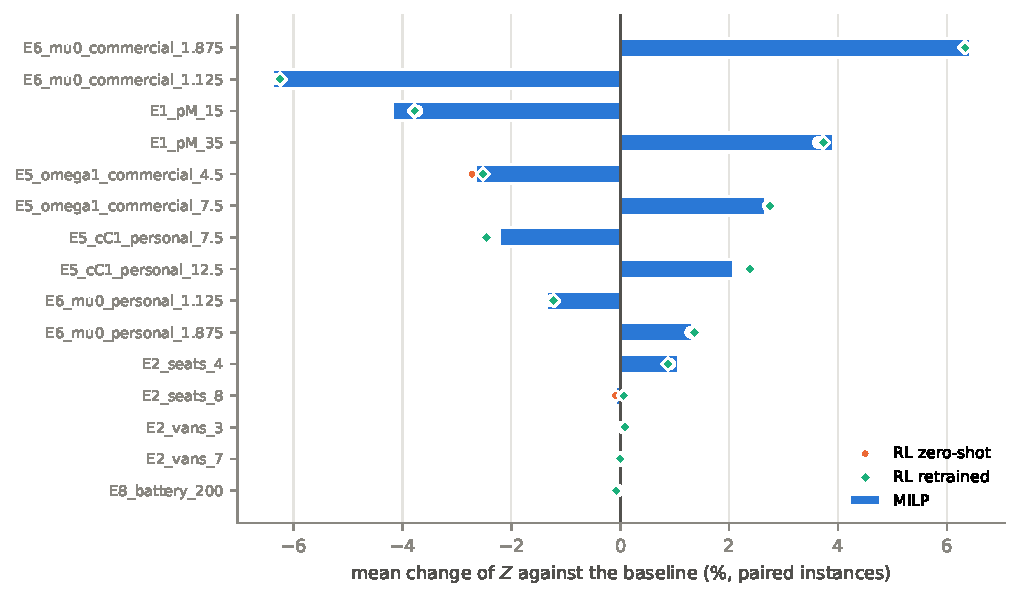
\includegraphics[width=0.9\textwidth]{figures/exp_tornado.pdf}
\caption{Mean change of $Z$ for every variant (bars: MILP; markers: RL, Part V). Sorted by size.}
\label{fig:tornado}
\end{figure}

Ranking by the effect on $Z$ of a $\pm25$\,\% or comparable change:
\begin{enumerate}
  \item commercial money sensitivity $\mu^0$: $\pm6.4$\,\%;
  \item van tariff $p^M$: $-4.2$ / $+3.9$\,\%;
  \item commercial downtime rate $\omega^1$: $\pm2.7$\,\%;
  \item personal value of station time $c^{C,1}$: $\pm2.1$\,\%;
  \item personal money sensitivity $\mu^0$: $\pm1.3$\,\%;
  \item seats per van (only when cut): $+1.1$\,\%;
  \item number of vans, battery: about 0\,\% (but the fleet decides feasibility).
\end{enumerate}
For \emph{who gets vans}, the ranking is different: the van tariff, the personal value of station time and cutting seats move the personal van share by about 6 to 12 percentage points; the money sensitivities and the commercial downtime rate move it by about 1 point or less.

\inshort{To estimate the cost well, measure how poor drivers feel money; to decide who gets vans, set the van tariff and know how much private owners value station time.}

\part{Results of reinforcement learning}
%=====================================================================
\section{RL baseline against the MILP}

\subsection{Valid plans, cost and speed}

\begin{table}[H]
\centering
\caption{RL baseline against the MILP baseline, by class. Gap = $100\,(Z_{\text{RL}}-Z_{\text{MILP}})/Z_{\text{MILP}}$ over instances where both plans are valid; s = mean seconds per instance.}
\small
\begin{adjustbox}{max width=\linewidth}
\begin{tabular}{@{}lrrrrrrr@{}}
\toprule
class & instances & MILP valid & RL valid & \shortstack{gap mean\\(\%)} & \shortstack{gap median\\(\%)} & MILP s & RL s \\
\midrule
C1 & 90 & 89 & 90 & 0.84 & 0.84 & 110 & 0.12 \\
C2 & 80 & 79 & 79 & 1.66 & 1.80 & 109 & 0.12 \\
R1 & 120 & 75 & 89 & 0.38 & 0.31 & 137 & 0.12 \\
R2 & 110 & 110 & 110 & 1.16 & 1.26 & 130 & 0.12 \\
RC1 & 80 & 42 & 52 & 0.12 & 0.33 & 171 & 0.12 \\
RC2 & 80 & 79 & 80 & 0.48 & 0.46 & 189 & 0.12 \\
\midrule
all & 560 & 474 & 500 & 0.85 & 0.76 & 140 & 0.12 \\
\bottomrule
\end{tabular}
\end{adjustbox}

\end{table}

\begin{itemize}
  \item \textbf{RL finds more valid plans}: \frlValid{} instances against the MILP's \fmilpValid. In \frlOnly{} instances RL has a valid plan where the MILP found none in 300 seconds (all of them ``time limit without a plan'' for the MILP); the reverse happens \fmilpOnly{} times. The \frlInvalid{} RL plans that are not valid include the \fmilpInfeasible{} provably infeasible instances, where no method can succeed.
  \item \textbf{RL plans cost a little more}: on the \frlPaired{} instances where both are valid, \frlGapMean\,\% more on average (median \frlGapMedian\,\%); against the instances the MILP proved optimal, \frlGapOpt\,\%. In \frlBetter{} instances RL is \emph{cheaper} than the MILP's time-limited plan.
  \item \textbf{RL is about a thousand times faster}: \frlSolveMean{} s per instance for 520 plans, against \fmilpSolveMean{} s for the MILP.
  \item \textbf{Where RL is closest}: the hard short-period classes R1 (0.38\,\%) and RC1 (0.12\,\%), exactly where the MILP struggles. \textbf{Where it is furthest}: C2 (1.66\,\%), long periods with clustered customers, where there are many possible orders and the MILP has time to find very good ones.
\end{itemize}

\begin{figure}[H]
\centering
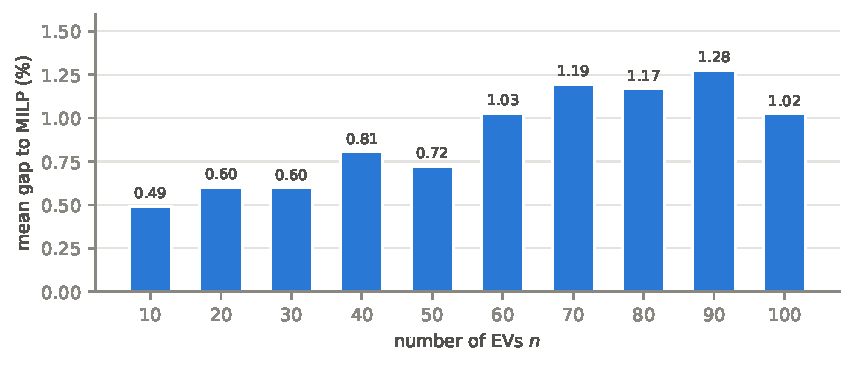
\includegraphics[width=0.85\textwidth]{figures/rl_gap_by_n.pdf}
\caption{Mean gap of RL to the MILP by instance size.}
\label{fig:rlgapn}
\end{figure}

The gap grows with size, from about 0.5\,\% at 10 cars to 1.2--1.3\,\% at 70--90 cars, and falls at 100 cars, where the MILP itself often stops far from optimal.

\inshort{RL gives a valid plan more often than the MILP, costs less than 1\,\% more on average, and needs a tenth of a second instead of more than two minutes.}

\subsection{Checks of the RL results}

All 31 RL runs (baseline + 15 variants $\times$ zero-shot and retrained) were checked file by file after the results were copied from the server:
\begin{itemize}
  \item every run has all 560 instances, each once, and no run ended with an error;
  \item a plan is marked valid exactly when it has no unplaced car and no violated rule;
  \item no RL plan is valid on an instance the MILP proved infeasible (that would be impossible);
  \item \code{plan.csv} has one row for every car of every instance;
  \item the comparison tables written on the server were recomputed from \code{runs.csv}: paired instances and mean change of $Z$ match exactly in all 30 experiment runs;
  \item an RL plan can never be cheaper than a proven optimum. Gurobi calls a plan optimal when it is within 0.01\,\% of the best possible; in 4 small instances (EV-C102 and EV-C103, 10--20 cars, in three variants) an RL plan is 0.0002--0.008\,\% cheaper than the MILP's ``optimal'' plan, i.e.\ inside that tolerance. Nowhere else;
  \item all 16 RL models are present; every training stopped early by the rule (epoch 210 or 211), with the best epoch between 145 and 201.
\end{itemize}

\inshort{The RL results are complete and consistent; the only oddity, four plans a hair cheaper than Gurobi's ``optimal'', is explained by Gurobi's 0.01\,\% optimality tolerance.}

\subsection{How RL's plans differ: it uses fewer vans}

The segment table of Part IV (and Figure~\ref{fig:vanincome}) shows the main difference in behaviour:
\begin{itemize}
  \item RL gives a van to only \fvanPersRl\,\% of free-choice personal cars, against \fvanPersMilp\,\% in the MILP plans; in the richest band 13\,\% against 41\,\%.
  \item The order is the same as the MILP's (van use rises with income for personal cars, almost zero for commercial cars), but much weaker.
  \item In exchange RL's customers queue longer at stations (commercial 3.4 against 1.6 minutes, personal 0.8 against 0.4).
\end{itemize}
Yet the cost is less than 1\,\% higher. So the cost is ``flat'' around the best plan: for a rich private owner, the van's advantages (no drive, faster charging, driver free) and its disadvantages (van premium, dearer van energy, dispatch cost) nearly balance, and moving such a customer from a van to a station changes $Z$ only a little.

Why does RL open fewer vans? Three likely reasons:
\begin{enumerate}
  \item \textbf{The dispatch cost comes first.} In the step-by-step construction, the first car put on a van carries the whole dispatch cost (Rs 1\,500) at that moment; the next five cars on the same van come almost free. The MILP sees the whole route at once. A policy that decides one car at a time sees opening a van as expensive.
  \item \textbf{Its teacher prefers stations.} The warm-up copies the greedy rule, which gives every car its cheapest option at that moment, usually a station.
  \item \textbf{Filling a van takes a coordinated series of choices}, which random sampling during training rarely finds.
\end{enumerate}
The same pattern was found for RL1 in formulation 3 (van share 3.6\,\% against the MILP's 7.0\,\%).

\inshort{RL reaches almost the same cost with a different plan: fewer vans, longer queues. This shows that many quite different plans are nearly equally good, and that RL's step-by-step view under-values opening a van.}

%=====================================================================
\section{RL experiments}

The RL rows are in the experiment tables of Part IV (Section~\ref{sec:milpexp}). Table~\ref{tab:expsummary} collects them.

\begin{table}[H]
\centering
\caption{All 15 variants: mean change of $Z$ (\%) with the MILP, RL zero-shot (ZS) and RL retrained (RT); valid plans; mean gap of RL to the MILP of the same variant (\%); training minutes and best epoch of the retrained model.}
\label{tab:expsummary}
\footnotesize
\begin{adjustbox}{max width=\linewidth}
\begin{tabular}{@{}lrrrrrrrrr@{}}
\toprule
variant & \shortstack{$\Delta Z$\\MILP} & \shortstack{$\Delta Z$\\RL-ZS} & \shortstack{$\Delta Z$\\RL-RT} & valid MILP & valid RL-RT & gap RL-ZS & gap RL-RT & train (min) & best epoch \\
\midrule
E5\_cC1\_personal\_7.5 & $-$2.21 & $-$2.49 & $-$2.46 & 473 & 500 & 0.56 & 0.56 & 38 & 201 \\
E5\_cC1\_personal\_12.5 & $+$2.08 & $+$2.45 & $+$2.38 & 473 & 500 & 1.22 & 1.14 & 39 & 200 \\
E5\_omega1\_commercial\_4.5 & $-$2.67 & $-$2.72 & $-$2.52 & 472 & 500 & 0.82 & 0.98 & 40 & 145 \\
E5\_omega1\_commercial\_7.5 & $+$2.66 & $+$2.72 & $+$2.75 & 475 & 499 & 0.83 & 0.86 & 39 & 148 \\
E6\_mu0\_personal\_1.125 & $-$1.35 & $-$1.28 & $-$1.22 & 473 & 501 & 0.92 & 0.95 & 39 & 188 \\
E6\_mu0\_personal\_1.875 & $+$1.33 & $+$1.29 & $+$1.36 & 475 & 499 & 0.80 & 0.84 & 40 & 180 \\
E6\_mu0\_commercial\_1.125 & $-$6.38 & $-$6.31 & $-$6.25 & 475 & 500 & 0.87 & 0.91 & 39 & 183 \\
E6\_mu0\_commercial\_1.875 & $+$6.43 & $+$6.34 & $+$6.33 & 475 & 500 & 0.80 & 0.79 & 38 & 200 \\
E1\_pM\_15 & $-$4.19 & $-$3.74 & $-$3.78 & 471 & 499 & 1.31 & 1.25 & 39 & 186 \\
E1\_pM\_35 & $+$3.91 & $+$3.64 & $+$3.73 & 477 & 500 & 0.58 & 0.64 & 40 & 148 \\
E2\_vans\_3 & $-$0.04 & $+$0.02 & $+$0.09 & 441 & 466 & 0.91 & 0.96 & 38 & 186 \\
E2\_vans\_7 & $+$0.02 & $+$0.04 & $+$0.00 & 487 & 506 & 0.84 & 0.81 & 38 & 181 \\
E2\_seats\_4 & $+$1.08 & $+$0.91 & $+$0.88 & 471 & 494 & 0.69 & 0.65 & 40 & 188 \\
E2\_seats\_8 & $-$0.08 & $-$0.08 & $+$0.07 & 471 & 499 & 0.85 & 0.98 & 38 & 162 \\
E8\_battery\_200 & $-$0.01 & $-$0.02 & $-$0.07 & 476 & 500 & 0.83 & 0.77 & 39 & 197 \\
\bottomrule
\end{tabular}
\end{adjustbox}

\end{table}

\subsection{Does RL measure the same effects as the MILP?}

\begin{figure}[H]
\centering
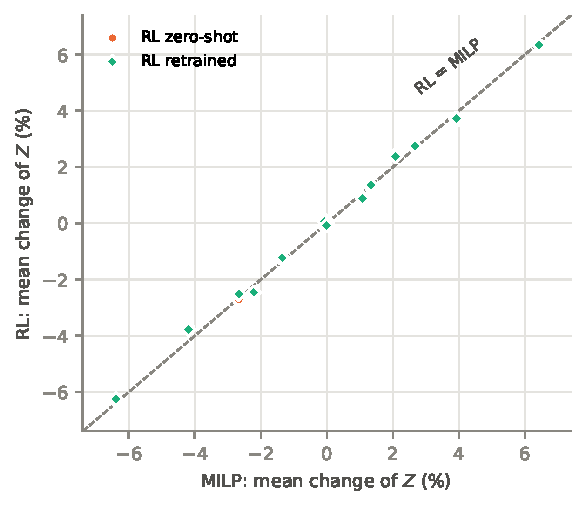
\includegraphics[width=0.55\textwidth]{figures/exp_agreement.pdf}
\caption{Change of $Z$ in each variant: MILP (horizontal) against RL (vertical). Points on the dashed line mean that RL measures exactly the MILP's effect.}
\label{fig:agree}
\end{figure}

\textbf{Yes, for the cost.} All points lie close to the line. On average the RL effect differs from the MILP effect by \fagreeZsMean{} percentage points (zero-shot) and \fagreeRtMean{} points (retrained). The direction agrees in \fagreeSign{} of \fnVariants{} variants; the two exceptions (3 vans, 8 seats) are the variants where the MILP effect itself is below 0.1\,\%, i.e.\ noise. The ranking of the assumptions (Figure~\ref{fig:tornado}) is the same with both methods.

\subsection{Does RL change who gets vans the same way?}

\begin{figure}[H]
\centering
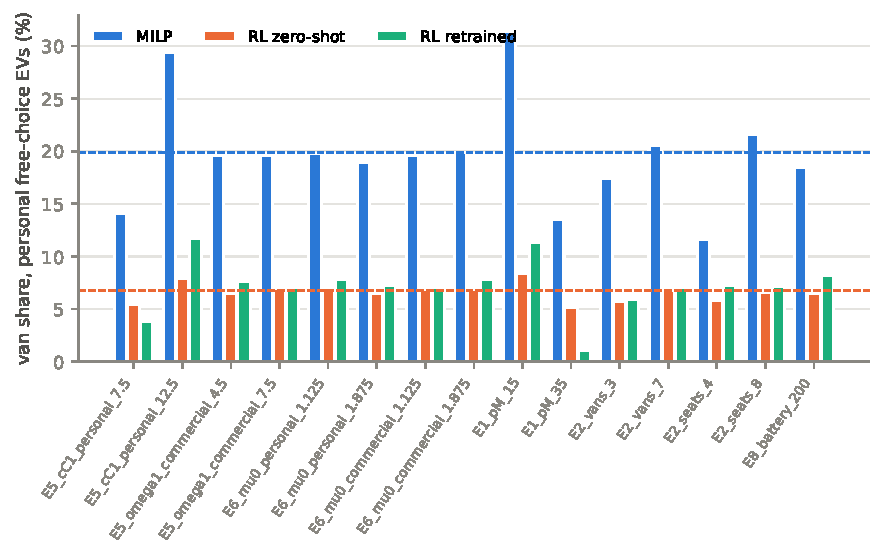
\includegraphics[width=0.95\textwidth]{figures/exp_vanshare.pdf}
\caption{Van share of free-choice personal cars in every variant. Dashed lines: the baselines (blue MILP, orange RL).}
\label{fig:expvan}
\end{figure}

\textbf{Only partly.} RL starts from a much lower van share (6.7\,\% against 19.9\,\%) and its response is weaker:
\begin{itemize}
  \item \textbf{E1 tariff}: no premium raises RL's personal van share to 8.4\,\% (zero-shot) or 11.3\,\% (retrained), the MILP's to 31.4\,\%; a doubled premium lowers it to 5.1\,\% or 1.1\,\% (MILP 13.5\,\%). Same direction, smaller size; the retrained policy reacts more than the zero-shot one.
  \item \textbf{E5 personal value of station time}: same direction (retrained 3.9\,\% and 11.7\,\%, MILP 14.1\,\% and 29.4\,\%).
  \item \textbf{E2 seats}: with 4 seats the MILP's van share falls from 19.8 to 11.6\,\%, RL's hardly moves: RL uses so few vans that the seat limit rarely binds for it.
  \item \textbf{E6 and commercial E5}: the MILP's van share does not move; the retrained policies vary by about $\pm1$ point around their baseline, which is training noise.
\end{itemize}

\subsection{Feasibility and quality in the variants}

\begin{figure}[H]
\centering
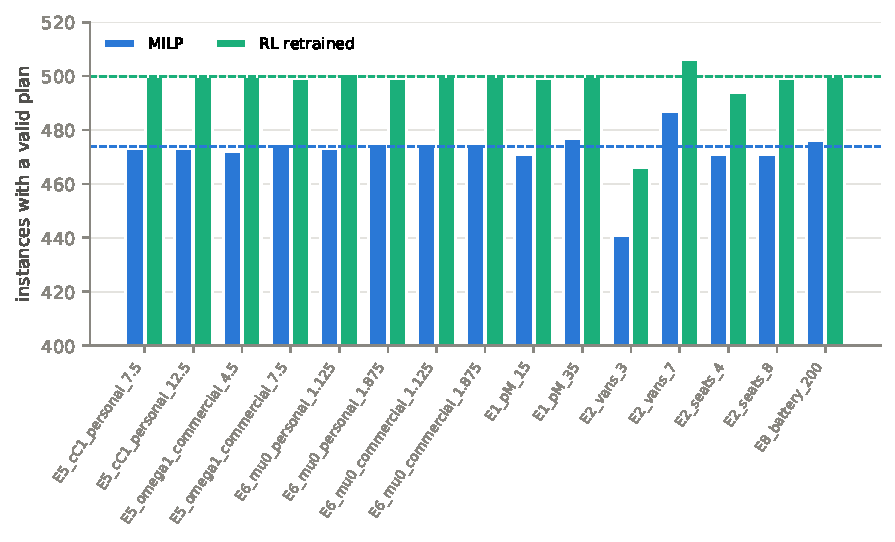
\includegraphics[width=0.95\textwidth]{figures/exp_valid.pdf}
\caption{Instances with a valid plan in every variant (dashed: the baselines).}
\label{fig:expvalid}
\end{figure}

\begin{itemize}
  \item RL has more valid plans than the MILP in every variant (465--506 against 441--487).
  \item The fleet effect is the same for both: with 3 vans RL loses 34--35 instances (MILP 33), with 7 vans it gains 6 (MILP 13).
  \item The gap to the MILP of the same variant stays between 0.56\,\% and 1.31\,\%. It is largest when vans become cheap (E1 $p^M=15$: 1.25--1.31\,\%) and smallest when they become less attractive (E5 personal 7.5: 0.56\,\%; E1 $p^M=35$: 0.58--0.64\,\%). This fits the explanation above: RL's weakness is opening vans, so it costs most when vans are worth most.
\end{itemize}

\subsection{Zero-shot or retrain?}

The zero-shot runs (baseline policy, no new training) are as good as the retrained ones: the gaps to the MILP differ by at most 0.16 points, and the measured effects on $Z$ by at most 0.2 points. Retraining took about 39 minutes per variant (15 models, best epochs 145--201). For $\pm25$\,\% changes of the customer numbers, tariff or fleet, \textbf{one trained policy can be reused without retraining}, because its inputs already contain the changed costs and fleet.

\inshort{RL measures the same cost effects as the MILP, within about 0.15 points, and keeps finding valid plans in every variant. It reacts to changes in van use in the right direction but much more weakly, because it opens few vans to begin with. Retraining is not needed for changes of this size.}

\part{MILP and RL side by side, and conclusions}
%=====================================================================
\section{MILP and RL side by side}

\begin{table}[H]
\centering\small
\caption{The two methods on the baseline (560 instances).}
\begin{tabular}{@{}lrr@{}}
\toprule
 & MILP (Gurobi, 300 s) & RL (attention policy) \\
\midrule
valid plans & \fmilpValid & \frlValid \\
proven optimal & \fmilpOptimal & -- (no proof) \\
instances with no plan & \fmilpTLnoPlan{} + \fmilpInfeasible{} infeasible & \frlInvalid{} (incl.\ the \fmilpInfeasible{} infeasible) \\
mean cost against the other & best & $+$\frlGapMean\,\% (median $+$\frlGapMedian\,\%) \\
mean time per instance & \fmilpSolveMean{} s & \frlSolveMean{} s \\
one-off cost & none & training \frlTrainMin{} min on a GPU \\
van share, personal free-choice cars & \fvanPersMilp\,\% & \fvanPersRl\,\% \\
van share, commercial free-choice cars & \fvanComMilp\,\% & \fvanComRl\,\% \\
mean station queue, commercial & \fqueueComMilp{} min & 3.36 min \\
experiment effects on $Z$ & reference & within about 0.15 points \\
\bottomrule
\end{tabular}
\end{table}

\textbf{When to use which.}
\begin{itemize}
  \item \textbf{For the best plan of one instance, and for proofs}, the MILP: it gives proven optima for half the instances and plans within a few per cent for most others, and it shows the true structure of a good plan (who should get vans).
  \item \textbf{For many instances, quick answers, or the hardest short-period cases}, RL: it answers in a tenth of a second, finds valid plans in 26 instances where the MILP found none, and measures the effect of a changed assumption almost exactly as the MILP does.
  \item \textbf{For the question ``who gets vans''}, rely on the MILP: RL's plans are almost as cheap but use far fewer vans, so its van shares should not be read as the best policy.
  \item \textbf{Together}: RL plans could be given to Gurobi as starting plans, exactly as the greedy plan is now; in the 26 instances where only RL found a plan, this would give the MILP a start it does not have today.
\end{itemize}

\inshort{The MILP is the reference for quality and for the structure of the plan; RL is the fast, robust tool, good enough to measure how the cost reacts to the assumptions.}

%=====================================================================
\section{Summary of findings}

\begin{enumerate}
  \item \textbf{Segment matters more than income for van use.} Personal cars get vans (19.9\,\% of those that can choose, 41\,\% of the richest); commercial cars almost never (0.7\,\%), and when they do, it is the poorest drivers escaping queues. This is exactly what the theory of formulation 4 predicted: the driver-free benefit belongs to private owners; taxis take vans only to save downtime.
  \item \textbf{Low-income customers absorb the queues}: commercial drivers queue about four times as long as private owners, and feel each rupee they pay much more.
  \item \textbf{$Z$ depends most on how poor drivers feel money} ($\pm6.4$\,\% for $\pm25$\,\% in $\mu^0_C$), then on the van tariff ($\pm4$\,\%), the downtime rate ($\pm2.7$\,\%) and the private owners' value of station time ($\pm2.1$\,\%). These are the numbers worth measuring better.
  \item \textbf{Who gets vans depends on the van tariff and the private owners' value of station time}; cheaper vans help mostly rich private owners and cost the operator more.
  \item \textbf{The fleet size decides feasibility, not cost}: with 3 vans 33 instances lose their plan, with 7 vans 13 gain one, while optimal costs do not move. Fewer seats per van raise the cost (+1.1\,\%).
  \item \textbf{The van battery is never the binding limit}: van recharging need not be modelled.
  \item \textbf{The results are internally consistent}: all 15 variants move the optimal cost in the direction the model requires (0 violations in about 4\,000 pairs of optimal plans), and the 51 infeasible instances are the same in every variant except 3 vans.
  \item \textbf{RL is a fast, reliable substitute for measuring costs} (valid plans in 500 instances, $+$0.85\,\% cost, about 1\,000 times faster, the same experiment effects), but it opens too few vans.
\end{enumerate}

%=====================================================================
\section{Limitations}

\begin{itemize}
  \item \textbf{Placeholders.} Apart from the segment share and the income distributions, the customer numbers are reasoned guesses. The experiments show how much each matters, not what the true value is.
  \item \textbf{One change at a time.} Interactions (for example cheaper vans \emph{and} more vans) are not tested.
  \item \textbf{Time limit.} 223 of 560 baseline instances end at the 300-second limit; effects smaller than the typical gap (a few per cent) are measured reliably only on the instances optimal in both runs, as in Table~\ref{tab:direction}.
  \item \textbf{Static demand.} All requests are known at the start. Real requests arrive during the day.
  \item \textbf{RL}: no optimality guarantee; one training run per model; under-uses vans; trained and tested only on the 100-car files.
  \item \textbf{Equity} is described (who queues, who pays, who feels what) but not part of the objective.
\end{itemize}

\section{Possible next steps}
\begin{enumerate}
  \item Measure the commercial money sensitivity and downtime rate, and the private owners' value of station time, with a small survey: they drive most of the results.
  \item Use RL plans as MILP starting plans, especially for R1/RC1.
  \item Make RL open vans more readily: spread the dispatch cost over the cars of a van in the training signal, or add active search per instance (as in RL2).
  \item Test combinations of changes (tariff with fleet) and a version with requests arriving during the day.
\end{enumerate}

%=====================================================================
\section*{Appendix: files and how to rebuild this report}
\addcontentsline{toc}{section}{Appendix: files and how to rebuild this report}

All in \code{2026-11-22\_formulation\_4/}:
\begin{itemize}
  \item \code{data/}: the dataset with segment and income; \code{data/calibration.md}: where the segment share and income distributions come from;
  \item \code{common/f4\_params.json}, \code{common/experiments.json}: customer parameters and experiments;
  \item \code{baseline\_MILP/}, \code{baseline\_RL/}, \code{<E>\_<name>\_MILP/}, \code{<E>\_<name>\_RL/}: code, results (\code{runs.csv}, \code{plan.csv}, \code{analysis/}, \code{comparison/}), RL models and logs;
  \item \code{job\_progress.log}: the server job, step by step (22--25 Nov 2026, all steps exit code 0);
  \item \code{report/}: this report. \code{make\_report\_f4.py} reads the results (nothing else) and writes \code{figures/}, \code{tables/} and \code{numbers.tex}; then \code{latexmk -pdf comprehensive\_report\_f4.tex}.
\end{itemize}


\end{document}
